\documentclass[german,12pt,paper=a4,DIV=calc,twoside, openright]{scrreprt}

%~ \usepackage[a-1b,latxmp]{pdfx}
\usepackage[T1]{fontenc}
\usepackage[utf8]{inputenc}
\usepackage[ngerman]{babel}

% Einzugsart
\setlength{\parindent}{0em} 
\setlength{\parskip}{2em}

% spacing for paragraphs but no indent
\usepackage[onehalfspacing]{setspace}

%****************
% define medatata
% found on: http://golatex.de/pdfx-bzw-pdf-a-oder-pdf-x-t4427.html
%________________
% pub
\newcommand{\projektname}{Systematische Bewertung von\\Blockchain-Implementierungen\\im Unternehmenskontext} %mit umbrüchen
\def\Title{Systematische Bewertung von Blockchain-Implementierungen im Unternehmenskontext}%Titel nach Absprache mir Betreuerin
\def\Subject{Abschlussarbeit zum Studium Wirtschaftsinformatik (Bachelor)}
\def\Keywords{Blockchain, Distributed Ledger Technology, BigchainDB, Quorum, Hyperledger, Bitcoin, Ethereum, Bewertung, Benchmarking}
%~ \def\Publisher{Hochschule für Technik und Wirtschaft Dresden (HTW Dresden)}
\def\Copyright{Creative Commons: Namensnennung und Weitergabe unter gleichen Bedingungen 4.0}
\def\CopyrightIMG{\includegraphics[width=2cm]{img/CC-BY-SA_icon}}
\def\CopyrightURL{https://creativecommons.org/licenses/by-sa/4.0/}

% priv
\InputIfFileExists{customize-priv}{}{
% if not
\def\Author{Autorennamen}
\def\AuthorID{00000}
\def\ReviewerA{Prof.~Dr. A}
\def\ReviewerB{Dipl.-Wirt.-Inf. B}
\def\SupervisorA{Dipl.-Inf. C}
\def\SupervisorB{}
\def\DocDate{\today}
\def\WritePlace{CityTownPlace}
\def\RepoURL{}
}
%\input{customize-priv}

\def\setRGBcolorprofile{sRGB_IEC61966-2-1_black_scaled.icc}
\def\setCMYKcolorprofile{coated_FOGRA39L_argl.icc}
%~ %***************************************************************************
% \convertDate converts D:20080419103507+02'00' to 2008-04-19T10:35:07+02:00
% found on: http://support.river-valley.com/wik.....ompliant_PDFs_from_pdftex
%___________________________________________________________________________
\def\convertDate{%
    \getYear
}
{\catcode`\D=12
 \gdef\getYear D:#1#2#3#4{\edef\xYear{#1#2#3#4}\getMonth}
}
\def\getMonth#1#2{\edef\xMonth{#1#2}\getDay}
\def\getDay#1#2{\edef\xDay{#1#2}\getHour}
\def\getHour#1#2{\edef\xHour{#1#2}\getMin}
\def\getMin#1#2{\edef\xMin{#1#2}\getSec}
\def\getSec#1#2{\edef\xSec{#1#2}\getTZh}
\def\getTZh +#1#2{\edef\xTZh{#1#2}\getTZm}
\def\getTZm '#1#2'{%
    \edef\xTZm{#1#2}%
    \edef\convDate{\xYear-\xMonth-\xDay T\xHour:\xMin:\xSec+\xTZh:\xTZm}%
}
 
\expandafter\convertDate\pdfcreationdate

\pdfinfo{%
    /Title    (\Title)
    /Author   (\Author)
    /Subject  (\Subject)
    /Keywords (\Keywords)
    /ModDate  (\pdfcreationdate)
    /Trapped  /False
    %~ /Publisher(\Publisher)
	/Copyright(\Copyright)
	/CopyrightURL(\CopyrightURL)
	/setRGBcolorprofile(\setRGBcolorprofile)
	/setCMYKcolorprofile(\setCMYKcolorprofile)
}


%~ \usepackage{lmodern}
%~ \PrerenderUnicode{äöüÄÖÜß}
%~ \usepackage[protrusion=true,expansion=true]{microtype} % Better typography

% needs to be (like) arial - uggly
%~ \usepackage[scaled]{helvet}
%~ \renewcommand*{\familydefault}{\sfdefault}

\usepackage[autostyle=true,german=quotes]{csquotes}
\usepackage[top=2cm,bottom=2.5cm,left=2.5cm,right=2.5cm]{geometry}
\usepackage{comment}
\usepackage{graphicx}
\usepackage{tikz}
%~ % Skalieren auf breite oder Höhe
\usepackage{environ}

\makeatletter
\newsavebox{\measure@tikzpicture}
\NewEnviron{scaletikzpicturetowidth}[1]{%
  \def\tikz@width{#1}%
  \def\tikzscale{1}\begin{lrbox}{\measure@tikzpicture}%
  \BODY
  \end{lrbox}%
  \pgfmathparse{#1/\wd\measure@tikzpicture}%
  \edef\tikzscale{\pgfmathresult}%
  \BODY
}
\NewEnviron{scaletikzpicturetoheight}[1]{%
  \def\tikz@width{#1}%
  \def\tikzscale{1}\begin{lrbox}{\measure@tikzpicture}%
  \BODY
  \end{lrbox}%
  \pgfmathparse{#1/\ht\measure@tikzpicture}%
  \edef\tikzscale{\pgfmathresult}%
  \BODY
}
\makeatother
\newlength{\imgwidth}
\newlength{\imgwidthmax}
\setlength{\imgwidthmax}{0.5\paperheight}
\newcommand\scalegraphics[1]{%
    \settowidth{\imgwidth}{\includegraphics{#1}}%
    \setlength{\imgwidth}{\minof{\imgwidthmax}{\minof{\imgwidth}{\textwidth}}}%
    \includegraphics[width=0.9\imgwidth]{#1}%
}

\usepackage{color}
%~ \usepackage{pdfpages}

% roman numbers support
\makeatletter
\newcommand*{\rom}[1]{%#1%
\expandafter\@slowromancap\romannumeral #1@%
}
\makeatother


% spacing of paragraphs influences lists, so fix that here 
%~ \usepackage{enumitem}
%~ \setlist[itemize]{parsep=0pt}
%~ \setlist[enumerate]{parsep=0pt}

% if we need listings for code or cli
%~ \usepackage{listings}
%~ \makeatletter
%~ \lst@Key{matchrangestart}{f}{\lstKV@SetIf{#1}\lst@ifmatchrangestart}
%~ \def\lst@SkipToFirst{%
    %~ \lst@ifmatchrangestart\c@lstnumber=\numexpr-1+\lst@firstline\fi
    %~ \ifnum \lst@lineno<\lst@firstline
        %~ \def\lst@next{\lst@BeginDropInput\lst@Pmode
        %~ \lst@Let{13}\lst@MSkipToFirst
        %~ \lst@Let{10}\lst@MSkipToFirst}%
        %~ \expandafter\lst@next
    %~ \else
        %~ \expandafter\lst@BOLGobble
    %~ \fi}
%~ \makeatother
%~ \definecolor{mygreen}{rgb}{0,0.6,0}
%~ \definecolor{mygray}{rgb}{0.5,0.5,0.5}
%~ \definecolor{mymauve}{rgb}{0.58,0,0.82}
%~ \lstset{ %
  %~ backgroundcolor=\color{white},   % choose the background color; you must add \usepackage{color} or \usepackage{xcolor}; should come as last argument
  %~ basicstyle=\ttfamily\footnotesize,        % the size of the fonts that are used for the code
  %~ breakatwhitespace=false,         % sets if automatic breaks should only happen at whitespace
  %~ breaklines=true,                 % sets automatic line breaking
  %~ captionpos=b,                    % sets the caption-position to bottom
  %~ commentstyle=\color{mygreen},    % comment style
  %~ deletekeywords={...},            % if you want to delete keywords from the given language
  %~ escapeinside={\%*}{*)},          % if you want to add LaTeX within your code
  %~ extendedchars=true,              % lets you use non-ASCII characters; for 8-bits encodings only, does not work with UTF-8
  %~ frame=single,	                   % adds a frame around the code
  %~ keepspaces=true,                 % keeps spaces in text, useful for keeping indentation of code (possibly needs columns=flexible)
  %~ keywordstyle=\color{blue},       % keyword style
  %~ language=Octave,                 % the language of the code
  %~ morekeywords={*,...},            % if you want to add more keywords to the set
  %~ numbers=right,                   % where to put the line-numbers; possible values are (none, left, right)
  %~ numbersep=5pt,                   % how far the line-numbers are from the code
  %~ numberstyle=\tiny\color{mygray}, % the style that is used for the line-numbers
  %~ matchrangestart=t,			   % show actual range from file
  %~ rulecolor=\color{black},         % if not set, the frame-color may be changed on line-breaks within not-black text (e.g. comments (green here))
  %~ showspaces=false,                % show spaces everywhere adding particular underscores; it overrides 'showstringspaces'
  %~ showstringspaces=false,          % underline spaces within strings only
  %~ showtabs=false,                  % show tabs within strings adding particular underscores
  %stepnumber=2,                    % the step between two line-numbers. If it's 1, each line will be numbered
  %~ stringstyle=\color{mymauve},     % string literal style
  %~ tabsize=2,	                   % sets default tabsize to 2 spaces
  %~ title=\lstname                   % show the filename of files included with \lstinputlisting; also try caption instead of title
%~ }
%~ \lstset{literate=
  %~ {á}{{\'a}}1 {é}{{\'e}}1 {í}{{\'i}}1 {ó}{{\'o}}1 {ú}{{\'u}}1
  %~ {Á}{{\'A}}1 {É}{{\'E}}1 {Í}{{\'I}}1 {Ó}{{\'O}}1 {Ú}{{\'U}}1
  %~ {à}{{\`a}}1 {è}{{\`e}}1 {ì}{{\`i}}1 {ò}{{\`o}}1 {ù}{{\`u}}1
  %~ {À}{{\`A}}1 {È}{{\'E}}1 {Ì}{{\`I}}1 {Ò}{{\`O}}1 {Ù}{{\`U}}1
  %~ {ä}{{\"a}}1 {ë}{{\"e}}1 {ï}{{\"i}}1 {ö}{{\"o}}1 {ü}{{\"u}}1
  %~ {Ä}{{\"A}}1 {Ë}{{\"E}}1 {Ï}{{\"I}}1 {Ö}{{\"O}}1 {Ü}{{\"U}}1
  %~ {â}{{\^a}}1 {ê}{{\^e}}1 {î}{{\^i}}1 {ô}{{\^o}}1 {û}{{\^u}}1
  %~ {Â}{{\^A}}1 {Ê}{{\^E}}1 {Î}{{\^I}}1 {Ô}{{\^O}}1 {Û}{{\^U}}1
  %~ {œ}{{\oe}}1 {Œ}{{\OE}}1 {æ}{{\ae}}1 {Æ}{{\AE}}1 {ß}{{\ss}}1
  %~ {ű}{{\H{u}}}1 {Ű}{{\H{U}}}1 {ő}{{\H{o}}}1 {Ő}{{\H{O}}}1
  %~ {ç}{{\c c}}1 {Ç}{{\c C}}1 {ø}{{\o}}1 {å}{{\r a}}1 {Å}{{\r A}}1
  %~ {€}{{\euro}}1 {£}{{\pounds}}1 {«}{{\guillemotleft}}1
  %~ {»}{{\guillemotright}}1 {ñ}{{\~n}}1 {Ñ}{{\~N}}1 {¿}{{?`}}1
  %~ {…}{{\ldots}}1 {–}{{--}}1
%~ }



%~ \usepackage[authoryear]{natbib}
% so:
\usepackage[backend=biber,%
citestyle=authoryear,%
urldate=comp,dateabbrev=false% for online sources date formatting
]{biblatex}
\addbibresource{quellen.bib}
\renewcommand{\bibfont}{\small}

% define string for bibliorphy urldate
%~ \DefineBibliographyStrings{english}{%
%~ urlseen = {Retrieved},
%~ }
\DefineBibliographyStrings{german}{%
urlseen = {Abgerufen},
}

% Glossar
\usepackage[ngerman]{translator}
%Paket laden
\usepackage[
nonumberlist, %keine Seitenzahlen anzeigen
acronym,      %ein Abkürzungsverzeichnis erstellen
toc,          %Einträge im Inhaltsverzeichnis
section]      %im Inhaltsverzeichnis auf section-Ebene erscheinen
{glossaries}
% Ein eigenes Symbolverzeichnis erstellen
\newglossary[slg]{symbolslist}{syi}{syg}{Symbolverzeichnis}
% Den Punkt am Ende jeder Beschreibung deaktivieren
\renewcommand*{\glspostdescription}{}
\makeglossaries

%~ \usepackage{bookmark}
%~ \hypersetup{%
	%~ draft,
	%pdfa,
	%unicode,
	%driverfallback=hpdftex,
	%hypertex,
	%colorlinks=false,pdfborderstyle={/S/U/W 1},% for non-PDF/A
	%~ colorlinks,
	%draft,%no links
	%~ allcolors=black,%for PDF/A with pdfx
%~ }
\usepackage{hyperref}

% minitoc
%~ \usepackage{minitoc}
% do not show minitoc error msgs
%~ \usepackage{silence}
%~ \WarningFilter{minitoc(hints)}{W0023}
%~ \WarningFilter{minitoc(hints)}{W0028}
%~ \WarningFilter{minitoc(hints)}{W0030}
%~ \WarningFilter{minitoc(hints)}{W0043}
%~ \WarningFilter{minitoc(hints)}{W0049}

% Kleiner Kommentar vor der bib, zitation funktioniert hierin nicht
\newcommand{\quellenHinweistext}{Online aufgefundene Quellen wurden via \href{https://archive.org/}{archive.org} gesichert und umfangreiche Werke bei Abgabe auf dem Datenträger beigelegt.}

% Glossareinträge einlesen
%Glossar-Einträge
\newglossaryentry{glos:Dezentralisierung}{
name=Dezentralisierung,
description={Als Gegensatz zur Zentralisierung. Hier insbesondere bezüglich Teilnehmern in Computernetzwerken bzw. Entscheidungsprozessen. Die Steigerung ist: Zentralisiert, Dezentralisiert, Verteilt.%
}}

\newglossaryentry{glos:MerkeTree}{
name=Merkle~tree,
description={Ein Baum -- aus durch seine Hashwerte rekursiv paarweise verbundenen Daten (die \enquote{Blätter}) -- mit genau einer Wurzel.%
}}

\newglossaryentry{glos:Chaincode}{
name=Chaincode,
description={Angelehnt an Smart~Contracts programmierbare Geschäftslogik mit gekapseltem State bei Hyperledger Fabric. Betroffene Teilnehmer müssen zustimmen.%
}}

\newglossaryentry{glos:Web3}{
name=Web3,
description={JavaScript API für Ethereum.%
}}

\newglossaryentry{glos:Fork}{
name=Fork,
description={Aufspaltung in einer Blockchain, die zur zeitweisen oder dauerhaften Spaltung führen kann.%
}}

\newglossaryentry{glos:Hard Fork}{
name=Hard Fork,
description={Vereinfacht: Nicht rückwärtskompatibel Protokolländerungen die ab einem bestimmten Block Gültigkeit erlangen.%
}}

\newglossaryentry{glos:Soft Fork}{
name=Soft Fork,
description={Vereinfacht: Rückwärtskompatibel Protokolländerungen die ab einem bestimmten Block Gültigkeit erlangen.}
}

\newglossaryentry{glos:SmartContract}{
name=Smart Contract,
description={Auch Chaincode (Firma IBM) genannte Programme, die auf einer Blockchain bzw. im Netzwerk der Teilnehmer laufen. Die Umsetzung erfolgt über einen Stack-basierte Programmierung deren Ergebnis den State beeinflusst. Z.B. Bitcoin durch das an Assembler erinnernde \enquote{Script} und bei Ethereum davon abstrahiert über höhere Programmiersprachen.}
}

\newglossaryentry{glos:State}{
name=State,
description={Hier der Zustand bezüglich einer Blockchain oder eines Smart~Contract.}
}

\newglossaryentry{glos:Block}{
name=Block,
description={Bildlicher Begriff für eine Datenstruktur, die Transaktionen zusammenfasst.}
}

\newglossaryentry{glos:FinTech}{
name=Financial Services and Technology,
description={Unternehmen, die mit Unterstützung von moderner Technologie Finanzdienstleistungen anbieten% \autocite{w:lexika-econimics}
}}

\newglossaryentry{glos:CR}{
name=Zensurresistenz,
description={Wie stark ein betrachteter Aspekt gegen Verschweigen, Löschen oder Veränderung geschützt ist.}
}

\newglossaryentry{glos:Konsens}{
name=Konsens,
description={Engl. Consensus. Hier die als Wahrheit angenommene, algorithmisch gesteuerte Aussagen wie Reihenfolge aber auch Zeit oder State in einem verteilten Netzwerk.
}}

\newglossaryentry{glos:Mining}{
name=Mining,
description={Englischer Begriff für \emph{Schürfen}. Ein Verfahren zum finden des nächsten Blocks, insbesondere bei Blockchains die auf Proof of Work basieren. Die Tätigkeit der Netzwerkteilnehmer wird damit bildlich dem Freilegen von seltenen  gleichgesetzt.}
}

\newglossaryentry{glos:Transaktion}{
name=Transaktion,
description={Datenstruktur, die ein Asset }
}

\newglossaryentry{glos:IRC}{
name=Internet Relay Chat,
description={Chatsystem, textbasiert. Seit 1993 durch die IETF als ein Internet Standard mit informationellem Charakter angenommen. s.a. \url{https://tools.ietf.org/html/rfc1459}}
}

\newglossaryentry{glos:PKI}{
name=Public-Key-Infrastruktur,
description={Ein System, das die Verteilung und Überprüfung von öffentlichen kryptografischen Schlüsseln unterstützt. In Unternehmen werden hierzu häufig Zertifikate nach dem Standard X.509 der \href{https://www.itu.int/}{Internationalen Fernmeldeunion} bzw. auch ISO/IEC\,9594-8 verteilt.}
}

\newglossaryentry{glos:PoW}{
name=Proof of Work,
description={Ein auf Hashcash %(s. Whitepaper \cite{p:bitcoin})
basierendes Verfahren, dass die Erstellung neuer Blöcke mit dem \emph{Ausgabeaufschlag} belohnt.% Die Schwierigkeit wird durch stetiges Suchen nach einem Ziel (z.B. Eigenschaft eines Hashes) steuert. Dieses Ziel kann u.a. durch die Anzahl der führenden Nullen %(s. \href{https://github.com/bitcoinbook/bitcoinbook/blob/8d01749bcf45f69f36cf23606bbbf3f0bd540db3/ch10.asciidoc\#proof-of-work-algorithm}{Proof of Work}% \autocite{b:mastering-bitcoin})
eines Hashes dargestellt werden, wie dies bei Bitcoin der Fall ist.%
}}

\newglossaryentry{glos:PoS}{
name=Proof of Stake,
description={Ein Konsensalgorithmen mit Anreizsystem durch einen riskierten Einsatz des eigenen Vermögens (z.B. an Kryptowährung). Ein Problem ist die zufällige Auswahl der über die Richtigkeit bestimmenden Teilnehmer für den jeweiligen Block. Teilweise wird dieser Ansatz durch Delegation zu \emph{delegated Proof of Stake} (dPoS) ergänzt.%
}}

\newglossaryentry{glos:Pruning}{
name=Pruning,
description={Engl. \emph{pruning}. Das Beschneiden/Zurechtstutzen, hier bezüglich der Einträge für Transaktionen in einem Block exkl. der Integritätsinformationen.%
}}

\newglossaryentry{glos:Schwierigkeit}{
name=Schwierigkeit,
description={Engl. difficulty, auch als Ableitung vom \emph{Ziel} (engl. target). Dient bei Konsens-Algorithmen für \gls{glos:PoW} zur Anpassung der Wahrscheinlichkeit des Entstehens eines neuen Blocks.
}}

\newglossaryentry{glos:Wallet}{
name=Wallet,
description={Entlehnt aus dem Engl. für Brieftasche als Bezeichnung für ein Programm, oder Datenstruktur bzw. Datei. Sie beinhaltet die kryptografischen Schlüssel für die Interaktion mit der Blockchain. 
}}

\newglossaryentry{glos:Ausgabeaufschlag}{
name=Ausgabeaufschlag,
description={Engl. blockreward. Die Belohnung für den Erfolgsfall bei einem Proof-of-Konsensmechanismus (s.a. Halfing).
}}

\newglossaryentry{glos:Exchange}{
name=Exchange,
description={Engl. für Wechslestuben. Hier Dienstleister und Märkte die dem Tausch zwischen stattlichen Währungen und Kryptowährungen/Token dienen.%
}}

\newglossaryentry{glos:Halfing}{
name=Halfing,
description={Halbierung des Ausgabeaufschlags (engl. \emph{Block Reward}) zur Regulierung der Gesamtmenge.
Bei Bitcoin wird der Ausgabeaufschlag (neue Bitcoin) alle 210.000 Blocks (d.h. statistisch etwa alle 4 Jahre) halbiert. \\
50 Bitcoin betrug der initiale Ausgabeaufschlag im Januar 2009.\\
25 Bitcoin ab \href{https://blockchain.info/block/000000000000048b95347e83192f69cf0366076336c639f9b7228e9ba171342e}{Block 210.000} am 28.11.2012\\% \autocite{w:blockchain}.
12,5 Bitcoin ab \href{https://blockchain.info/block/000000000000000002cce816c0ab2c5c269cb081896b7dcb34b8422d6b74ffa1}{Block 420.000}) am 09.07.2016\\% \autocite{w:blockchain}.
Kommende Halbierungen werden über verschiedene Webseiten (u.a. \url{http://www.thehalvening.com/} o. \url{http://bitcoinclock.com/}) nach Auswertung der Entwicklung der Schwierigkeit im Netzwerk geschätzt. \\
Bei Ethereum ist die absolute Menge nicht final festgelegt (\url{https://ethereum.stackexchange.com/questions/443/what-is-the-total-supply-of-ether}), andere native Währungen (z.B. \href{http://dogecoin.com/}{Dogecoin} oder \href{http://www.monero.cc/}{Monero}) haben teilweise eine infinite Menge.
}}

\newglossaryentry{glos:Hashrate}{
name=Hashrate,
description={Die Anzahl der Hashes je Zeiteinheit (meist je Sekunde). Die Absolute Zahl der Hashes wird äquivalent zur verrichteten Arbeit verstanden. Einerseits eine Maßzahl für die erbrachte Leistung eines einzelnen Teilnehmers. Zumeist aber die aufgrund der Schwierigkeit geschätzte Gesamtleistung des Netzwerkes.}
}

\newglossaryentry{glos:GenesisBlock}{
name=Genesis Block,
description={In Anlehnung an die griechische Bedeutung Schöpfung/Geburt -- u.a. bekannt durch das 1. Buch Mose der Bibel -- der erste Block einer Blockchain. Dieser wird üblicherweise vom Initiator unabhängig vom Mining erstellt.}
}

\newglossaryentry{glos:TPS}{
name=Transaktionsgeschwindigkeit,
description={Metrik für die Anzahl je Zeiteinheit durchführbarer oder tatsächlich durchgeführten Transaktionen nach Konsens.}
}

\newglossaryentry{glos:LN}{
name=Lightning Network,
description={Ein Netzwerk für das Routing von zunächst primär Zahlungstransaktionen im Bitcoin-Netzwerk und potentiell darüber hinaus beliebige Transaktionen über verschiedene Blockchains hinweg.
Die Erweiterung erfolgt als zweite Protokollschicht über Timelocks und Multisignature-Adressen in einem Smart~Contract. Wiederverwendbare Payment~Codes die die Handhabung von Adressen erleichtern und gleichzeitig den Datenschutz verbessern werden integriert.%
}}

%Abkürzungen
\newacronym{BTC}{BTC}{Bitcoin%
}
%Eine Abkürzung mit Glossareintrag
\newacronym{IRC}{IRC}{Internet Relay Chat\protect\glsadd{glos:IRC}
}
\newacronym{DNS}{DNS}{Domain Name System%\protect\glsadd{glos:AD}
}

\newacronym{DGN}{DGN}{Deutsches Gesundheitsnetz%\protect\glsadd{glos:AD}
}

\newacronym{DFN}{DFN}{Deutsches Forschungsnetz%\protect\glsadd{glos:AD}
}

\newacronym{PKI}{PKI}{Public-Key-Infrastruktur\protect\glsadd{glos:PKI}
}

\newacronym{LN}{LN}{Lightning Network\protect\glsadd{glos:LN}%
}

\newacronym{PoW}{PoW}{Proof of Work\protect\glsadd{glos:PoW}
}

\newacronym{PoS}{PoS}{Proof of Stake\protect\glsadd{glos:PoS}
}

\newacronym{TPS}{TPS}{Transaction Processing System\protect\glsadd{glos:TPS}%
}

\newacronym{GRNET}{GRNET}{Greek Research and Technology Network%
}

\newacronym{JSON}{JSON}{JavaScript Object Notation%
}

\newacronym{MQTT}{MQTT}{Message Queuing Telemetry Transport%MQTT ist ein offenes Nachrichtenprotokoll für Machine-to-Machine-Kommunikation, das die Übertragung von Telemetriedaten in Form von Nachrichten zwischen Geräten ermöglicht, trotz hoher Verzögerungen oder beschränkten Netzwerken.
}

\newacronym{IoT}{IoT}{Internet of Things%
}

\newacronym{DLT}{DLT}{Distributed-Ledger-Technologie%
}

\newacronym{BC}{BC}{Blockchain%
}

\newacronym{BCT}{BCT}{Blockchain-Technologie%
}

\newacronym{DAG}{DAG}{Directed Acyclic Graph%
}

\newacronym{DApp}{DApp}{Distributed App(lication)%
}

\newacronym{MIT}{MIT}{Massachusetts Institute of Technology%
}

\newacronym{HSM}{HSM}{Hochschule Mittweida%
}

\newacronym{EEA}{EEA}{Enterprise Ethereum Alliance%
}

\newacronym{ANS}{ANS}{Antshares%
}

\newacronym{BCI}{BCI}{Blockchain-Implementierung%
}

\newacronym{HTW}{HTW}{Hochschule für Technik und Wirtschaft Dresden%
}

\newacronym{MOOC}{MOOC}{Massive Open Online Course%
}

\newacronym{IPDB}{IPDB}{Interplanetary Database%
}

\newacronym{IPFS}{IPFS}{Interplanetary Filesystem%
}

\newacronym{VDI}{VDI}{Verein Deutscher Ingenieure% (\href{https://www.vdi.de}{vdi.de})%
}

\newacronym{OB}{OB}{OpenBazaar%
}

\newacronym{ICO}{ICO}{Initial Coin Offering%
}

\newacronym{SE}{SE}{Sharing Economy%
}

\newacronym{IDE}{IDE}{Integrated Development Environment%
}

\newacronym{FSF}{FSF}{Free Software Foundation%
}

\newacronym{OSI}{OSI}{Open Source Initiative%
}

\newacronym{OSD}{OSD}{Open~Source Definition%
}

\newacronym{RPC}{RPC}{Remote Procedure Call%
}

\newacronym{REST}{REST}{Representational State Transfer (seltener ReST)%
}

\newacronym{BCCM}{BCCM}{Blockchain Competence Center Mittweida%
}

\newacronym{PBC}{PBC}{Permissioned Blockchain%
}

\newacronym{HAWG}{HAWG}{Hyperledger Architecture Workgroup%
}

\newacronym{GPM}{GPM}{Geschäftsprozessmanagement%
}

\newacronym{BFT}{BFT}{Bycantine Fault Tolerance (Byzantine Fehlertoleranz)%
}

\newacronym{DRM}{DRM}{Digitales Rechte Management (engl. Digital Restrictions Management / Digital Rights Management)%
}



\begin{document}

% add bookmark for title page to pdf
%~ \pdfbookmark{Titelseite}{title}
\begin{titlepage}
\pagestyle{empty}

\hspace{1cm}\\
\,
\vspace{1cm}

\centering

	{
		\scshape
			\Huge \projektname{}
		\par
	}

\vspace{2cm}

{	\scshape	{\LARGE Bachelorarbeit Wirtschaftsinformatik} }

	\vspace{1mm}
	{		\small{an der}\\	}
	\hspace{1cm}\\
	\,
	\vspace{1em}
	{\includegraphics[width=5cm]{img/htw-logo}
\\%	\vspace{1mm}
	{	\large	Hochschule für Technik und Wirtschaft Dresden\\ }
	}

\vfill
	\vspace{2em}


\begin{tabular}{ll}% todo: conditionalize, add properties such as function, title
	Autor: & \Author{} \\
	Matrikelnummer: & \AuthorID{} \\
	Abgabedatum: & \DocDate{} \\
	& \\
	1. Gutachter: & \ReviewerA{} \\
	2. Gutachter: & \ReviewerB{} \\
	%1.
	Fachbetreuerin: & \SupervisorA{} \\
	%2. Fachbetreuer: & \SupervisorB{} \\
	
\end{tabular}

\par

\newpage

\hspace{1cm}\\
\,
\vspace{1cm}

\par

\vspace{1em}

\par



\vfill

\centering

%%
%~ \textbf{Lizenzbestimmungen} \vspace{0.5ex}

\CopyrightIMG{}

\Copyright{}\\
\url{\CopyrightURL}

\RepoURL{}
%%
\newpage

\end{titlepage}


%<Chap1…

\hspace{1em}\,\vspace{3em}
\addsec{Kurzfassung}
\pagenumbering{roman}
\setcounter{page}{1}
%\pagestyle{empty}

Durch diese Abschlussarbeit soll ein Verfahren für die Bewertung verschiedener, auch neu erscheinender, Blockchain-Implementierungen für Unternehmen entworfen werden.
Das Vorgehen soll als wiederholbarer Ansatz im Rahmen des betrieblichen Benchmarking die Auswahl vorab und auch den Vergleich, \zB{} nach eigenen Testläufen oder der Einführung einer Blockchain-Implementierung, unterstützen.
Dazu werden -- vor dem Hintergrund der beiden großen öffentlichen, globalen und erlaubnisfreien Blockchains Bitcoin und Ethereum -- beispielhaft Anwendungsfälle und einzelne andere Implementierungen betrachtet und Eigenschaften qualitativ als Kriterien herausgearbeitet. Zum Abschluss wird die Darstellung der Vergleichswerte in einer für Präsentationen und Entscheidung geeignete Form behandelt. 

%Abstract
%engl. transl.
 \newpage
%/Chap1>
\cleardoublepage 
%~ \pagenumbering{roman}
%~ \pagestyle{plain}

% add bookmark for toc to pdf
\pdfbookmark{\contentsname}{toc}

\tableofcontents
\cleardoublepage 

%Glossar ausgeben
\printglossary[style=altlist,title=Glossar]
\clearpage 
 
%Abkürzungen ausgeben
\deftranslation[to=German]{Acronyms}{Abkürzungsverzeichnis}
\printglossary[type=\acronymtype,style=long]
 
%Symbole ausgeben
%~ \printglossary[type=symbolslist,style=long]\cleardoublepage 

%~ \,
%~ \vspace{30em}
%~ {
%~ \LARGE\textbf{Danksagung}\vspace{1em}
%~ }

%~ Ich möchte mir herzlichst für die Geduld und Unterstützung bedanken,
%~ die mir sowohl beim ZIH aber auch von Seiten Thomas Jejkal, Entwickler
%~ des KIT Datamanager am Karlsruher Instutut für Technologie, entgegen
%~ gebracht wurde.

%~ \newpage

\pagenumbering{arabic} %for actual content

%<Chap1…
% Umfang 40-60 Seiten (15-30 / Monat)

%~ Thema => Ausgangsproblem => Forschungsfrage
%~ Einführung => Auslöser, Verlauf, Ergebnis
%~ Kern => Forschungsfrage behandeln => Eigenleistung, nicht nur allg. Sachverhalte wiedergeben
%~ Hypothemen => Begründete Annahme => Was sind die Unklarheiten
%~ Arbeitsmethoden => Fragetsellungen => Quellen => Interview, Literatur, Experten, Kompetenzträger
%~ Theorien => Belegen Hypothesen => Plausible Erklärungsansätze
%~ Abschluss => Bogen zum Anfang spannen => Hypothesen bestätigt/verworfen

%~ \chapter{Einleitung}\label{einleitung}

%~ \emph{betonter text}
%~ \footnote{fußtnotentext}

%Abkürzungsverzeichnis

%Abbildungs- und Tabellenverzeichnisse

%Textteil

\chapter{Einleitung}\label{einleitung}

% warum relevant?

Der erste weltweit bekannte Vertreter der \emph{Blockchain}-Technologie war der im Jahr~2008 vorgestellte und seit Januar~2009\footnote{3.\,Januar~2009, \gls{glos:GenesisBlock} \autocite{w:bitcoin-wiki}} aktive \emph{Bitcoin}\footnote{s.a. \enquote{Bitcoin Whitepaper} \autocite{p:bitcoin}}.
Der sehr beschränkte primäre Einsatzzweck als \enquote{digitales Bargeld} über ein offenes, global verteiltes, zensurresistentes, transaktionsbasiertes\footnote{in Anlehnung an einen Vergleich von Andreas Antonopoulos bezüglich der Innovation von Bitcoin und der des Internet, \autocite{o:open-blockchain}} Peer-to-Peer-Netzwerk  wurde unlängst weiter gedacht und auf andere Anwendungszwecke, wie \zB{} seit Mitte Oktober~2010 Namecoin als DNS-Alternative (IRC\footnote{Transcript of bitcoin-dev channel \autocite{w:irc-ts-bitcoindev}}/Bitcointalk\footnote{\cite{w:bitcointalk-bitdns}}), ausgedehnt die ihrerseits auf einer Buchhaltung, Nachweisliste, einem Register o.ä. zentralen Vertrauensankern beruhen.

Das Problem, welches hier gelöst wurde, ist der \gls{glos:Konsens} in einem verteilten Netzwerk ohne Vertrauen auf eine zentrale Autorität oder explizite Erlaubnis\footnote{Tatsächlich gibt es Ausschlüsse als Strafmaßnahme für Spam oder vom Protokoll abweichendes Verhalten} der anderen Teilnehmer; bekannter als \enquote{Byzantinischer Fehler}\footnote{engl. \enquote{Byzantine Fault Tolerance} o. \enquote{Byzantine Generals Problem} \autocite{p:byzantine-original}}.
Dabei wird die Reihenfolge der Blöcke, und damit der darin befindlichen Transaktionen, unveränderbar.\footnote{nicht zwangsläufig zutreffend für den Inhalt, soweit ein Löschen durch kryptografische Maßnahmen ermöglicht wird \autocite{w:accenture-patent}}
Im Ergebnis werden Abweichungen vom Konsens durch andere Teilnehmer im Netzwerk als Regelverstoß erkannt und bestraft.
Die Einhaltung des Protokolls wird so wirtschaftlich erzwungen ohne einen Erlaubnisvorbehalt zu benötigen.
%~ Bisherige Ansätze wie Paxos\footnote{Voraussetzung ist die Position als Legislator \autocite{p:paxos}} waren dahingehend unvollständig.

%~ Tatsächlich ist die Forschung um die Konsens-Findung bereits wesentlich älter.
%~ Bereits in den 1980er Jahren wurde eine Reihe an Protokollen unter dem Namen Paxos veröffentlich, die noch heute in definierten Umgebungen das Problem 

Gleichartige Probleme sind in Unternehmen nicht nur in der Finanzbuchhaltung relevant.
Stets gibt es Gefälle von Vertrauen.
Zwischen
einfachen Mitarbeitern und Vorgesetzten,
zwischen Mitarbeitern mit bestimmten Verantwortungen gegenüber anderen Mitarbeiten
und nicht zuletzt
zwischen Vertragsparteien wie \zB{} Beteiligten aus unterschiedlichen Unternehmen bis hin zu Kunden.
Gleichzeitig steht die ökonomische Realität einem teilweise ideologisch geprägten verteilten, öffentlichen, erlaubnisfreien Idealbild entgegen.

% Damit ermöglicht ein solches System eine hochdynamische Menge an Teilnehmern im Netzwerk.
% durch einen ständigen Akkreditierungsprozess zur Prüfung der Teilnehmer 

Bereits im Jahr~2012 hat sich die \emph{Bitcoin Foundation} formiert, um in Wirtschaft und Politik für die vielfältig möglichen und legitimen Anwendungsfälle zu werben.
Das Unterfangen war bis heute von wenig Erfolg außerhalb der USA gekrönt.
Auch die Gründung des \emph{Bundesverband Bitcoin e.V.}\footnote{Website \url{https://www.bundesverband-bitcoin.de/}} in Deutschland war noch kaum mit dem erhofften Einfluss auf die Politik gesegnet.
Ende des Jahres~2015 hat die \emph{Linux Foundation} das Projekt \emph{Hyperledger} aufgenommen, Ethereum hat die \gls{EEA}\footnote{%Website \url{https://entethalliance.org/}
\cite{p:eea}} ausgegründet und ist inzwischen die größte Blockchain-Initiative\footnote{\cite{w:eea:launch}}.
Und auch in Deutschland sind mit dem \emph{Blockchain Bundesverband}\footnote{Website \url{http://bundesblock.de/}} inzwischen 19~Unternehmen -- zumeist Start-ups und mehrheitlich aus Berlin -- versammelt.

Unternehmen suchen bereits aktiv nach Arbeitnehmern im Umfeld der \emph{Blockchain}.
Darunter sind nicht nur \gls{glos:FinTech}, Banken, Beratungsfirmen und Start-ups, sondern auch Telekommunikationskonzerne, Automobilkonzerne und -Zulieferer, Reiseunternehmen, Brangenverbände, Energiekonzerne und Rüstungsindustrie.\footnote{\cite{w:jobsearch-bc-stepstone}}
Je Job-Portal kommen auf den Suchbegriff \enquote{Blockchain} zwei- bis dreistellige Trefferzahlen.
Allein auf dem regionalen Portal \href{https://www.itsax.de/}{ITsax.de} gibt es aktuell 10~Treffer\footnote{\cite{w:jobsearch-bc-itsax}}.

Auch Universitäten und Hochschulen widmen sich zunehmend dem Thema. Nikosia bietet \ua{} seit 2015 einen \gls{MOOC} und einen \enquote{Master of Science in Digital Currency}\footnote{3 Semester Fernstudium \enquote{Digital Currency} \autocite{w:unic-master-dc}} an. Auch Edinburgh, das \mbox{University College} London, Stanford, Berkeley, die \mbox{John Hopkins University}, das \gls{MIT} und Princeton bieten Studienkurse oder Module zum Thema an. 
Seitens der \gls{HSM} wurde im Jahr~2017 das \gls{BCCM}\footnote{Website \autocite{w:bccm}} initiiert. Dort wird auch die Zusammenarbeit hinsichtlich der Forschung zum des Einsatzes von \gls{BC} mit der Politik und Wirtschaft fachübergreifend angegangen.

\newpage
%%%
\section{Ausgangssituation und Problemstellung}\label{sec:problemstellung}
%%%
%Ausgangssituation und Problemstellung

Es gibt insbesondere seit Ende des Jahres~2013\footnote{s.a. \enquote{Ethereum Whitepaper} \autocite{p:ethereum}} zahlreiche Vertreter im Umfeld dieser speziellen Datenbank-Technologie.
Die viel diskutierte Anwendung für die Finanzierung von Unternehmungen mit einem \gls{ICO} und die damit einher gehenden meist spekulativ getriebenen Wertsteigerungen im Jahr~2017 bringt viel Aufmerksamkeit auch durch die Politik ein.
Eine weitere Auswirkung ist auch der Entwurf immer neuer Anwendungsfälle für die \gls{BCT}.
Unternehmen stehen im Zusammenhang mit den eigenen Prozessen und neuen Geschäftsideen vor der Herausforderung neu erscheinende \gls{BCI} zu bewerten um selbst Auswahl treffen zu können.
Hierzu sollen im Rahmen der Arbeit einzelne am Markt vertretene Blockchain-Implementierungen, in wiederholbarer und auf weitere Neuentwicklungen anwendbarer Weise, betrachtet werden.

\section{Ziel der Arbeit}

%~ Mein Arbeitsauftrag leitet sich aus dem Vertrag mit der T-Systems Multimediasolutions und der daraus resultieren Vereinbarung mit der \gls{HTW} ab.\footnote{Reihenfolge und Formulierung teilw. abweichend von }

Es soll ein System zur Bewertung von \gls{BCI} entworfen werden.
Die dafür notwendigen Kriterien sollen schrittweise recherchiert werden.
Dazu soll die Betrachtung von Anwendungsfällen sowie bestehender \gls{BCI} dienen.
Gefundene Kriterien müssen im Kontext der Bewertung und Darstellung quantifizierbar gestaltet sein.
Die Frage der Darstellung soll hinsichtlich der Unterstützung von Präsentation und Entscheidungsprozessen behandelt werden.

%~ \begin{enumerate}
%~ \item Herausstellen des Nutzens der Blockchain-Technologie für ausgewählte Anwendungsfälle im Unternehmenskontext
%~ \item Auswahl von mindestens drei am Markt konkurrierenden Kandidaten für Blockchain-Implementierungen
%~ \item Ermittlung und Analyse der Eigenschaften, die diese Kandidaten ausmacht
%~ \item Bewertung zum Zweck einer übersichtlichen Darstellung des Vergleiches
%~ \item Systematische Vorgehensweise anwendbar auf weitere zuvor nicht betrachtete Blockchain-Implementierungen
%~ \end{enumerate}

\section{Abgrenzung}\label{sec:abgrenzung}

Begrifflich wird die \gls{DLT} (auch Shared Ledger) als eine Datenbanktechnologie verstanden.\footnote{\enquote{What is a shared ledger?} \autocite{b:gos-dlt}}
Darunter verstehen wir neben der \gls{BCT}, die teilweise synonym verwendet wird, auch Ideen eine andere oder keine feste Anordnung der Datenobjekte in Blöcken vorzunehmen solange sie dazu keine zentrale Autorität, zentrale Speicher oder einen Erlaubnisvorbehalt benötigen und die Verfügbarkeit durch das Netzwerk gewährleistet wird.
Ein weiterer bekannter -- bislang theoretischer -- Vertreter ohne Blockchain und ohne Blöcke ist der Tangle bzw. \gls{DAG}\footnote{\enquote{DAG (Tangle) is not Blockchain} \autocite{w:satoshiwatch-dag}}.
Die bekannteste \gls{DAG}-Implementierung unter dem Namen \href{https://iota.org/}{IOTA}\footnote{\enquote{The Tangle} \autocite{p:iota}} läuft bisher jedoch nicht ohne einen zentrale Autorität\footnote{Ein Entwickler bestätigte den Umstand auf Nachfrage \autocite{w:iota-centralized}} -- den Koordinator der auch einen zentralen Speicher darstellt.
% Hashgraph\footnote{\href{https://hashgraph.com/}{hashgraph.com}} ist ein weiterer Ansatz ohne Blöcke mit einigen Einschränkungen
Die im Rahmen der Arbeit besprochene Form ist daher ausschließlich die bereits über Jahre bewährte \gls{BCT}.

% virtuelle Währung, Kryptowährung
Virtuelle Währungen (engl. Virtual Currency) benötigen keine \gls{BC}.
Virtuelle Währung gewinnen neue Eigenschaften wenn sie als (native) Kryptowährung (engl. Cryptocurrency) einer \gls{BC} verwendet werden.
Sie bieten einen Anreiz zur Einhaltung des Protokolls oder können wie im Fall von Ethereum den State einer \gls{DApp} verändern.
%~ Sie können eine maximale bzw. auch algorithmisch gesteuerte Geldmenge aufweisen. %Das Vertrauen der Bürger in den Staat ist sehr begrenzt wenn Währungskrisen auftreten.
Durch die Möglichkeit die Geldmenge algorithmisch zu steuern sind Kryptowährungen hinsichtlich der Geldmenge transparenter\footnote{Angaben zur Geldmenge \zB{} auf Coinmarketcap \autocite{w:cmc}} als Geldmengenberichte\footnote{Keine Aussage zur gesamten Geldmenge \autocite{w:ecb-moneydev}} der Zentralbank.
Neben diesen nativen Währungen kann \ua{} durch die Eigenschaft der Programmierbarkeit dieses Geldes weitere sog. Token\footnote{\enquote{What is An Ethereum Token} \autocite{w:eth-token}} oder Colored Coins\footnote{Colored Coins \autocite{b:mastering-bitcoin}%, \url{https://github.com/bitcoinbook/bitcoinbook/blob/8d01749bcf45f69f36cf23606bbbf3f0bd540db3/colored_coins.asciidoc}
} erstellt werden.
Auch ohne native Kryptowährung sind diese Möglichkeiten gegeben, lediglich der Anreiz zur Beteiligung an der \gls{BC} wäre dann ein anderer und die Frage nach der Verteilung der Token auf.
%~ Eine Möglichkeit für den Einsatz von Kryptowährungen ist der Betrieb von \gls{DApp} vorzusehen.
%~ Die Eigenschaften die zur Nutzbarkeit von Kryptowährungen führen sind damit Bestandteil der Arbeit. Nicht Bestandteil sind Fragen zu Legalität, Legitimität, Handel und anderen Gesichtspunkten der Finanzwirtschaft.

Die später näher betrachteten \gls{BCI} sollen durch ein Verfahren bewertet werden.
Sie sind damit Objekte der Bewertung.
Die Beurteilung der Objekte soll anhand konstituierender Eigenschaften stattfinden.\footnote{\cite{b:strassert:entscheidungen}}
Diese Eigenschaften nennen wir Kriterien für unsere Entscheidung.

\section{Methode}

Diese Arbeit basiert auf qualitativer Recherche unter Nutzung von Sekundärforschung, Forschungsüberblick, Betrachtung von Anwendungsfällen und bestehenden \gls{BCI} um Kriterien für die Beurteilung aufzufinden.
Damit wird der Herausforderung stetig neuer Veröffentlichungen um die Technologie Rechnung getragen, da die Forschung dazu noch nicht abgeschlossen und durch neue Ansätze geprägt ist.

Um mehr über die Grenzen der \gls{BCT} zu erfahren sollen Anwendungsfälle betrachtet werden, die eine Eignung für den Unternehmenseinsatz aufweisen.
Als allgemeine Annahme wird verfolgt, dass technologische Grenzen durch eine konkrete Implementierung entweder deutlich oder aber von der Implementierung abgemildert werden.
%Sofern solche Grenzen erkannt werden können, eignen sie sich als Kriterium für den Vergleich über verschiedene \gls{BCI} hinweg.
%D.h. über bekannt gewordene Anwendungsfälle sollen Kriterien ermittelt werden, die als Vor-/Nachteilen der \gls{BCT} oder der \gls{BCI} erkannt werden können.
Die theoretischen Vorteile werden bei der Werbung für Produkte üblicherweise stark betont, weshalb hier insbesondere auf Schwächen geachtet werden soll.

\textbf{Hypothese~\rom{1}} Anwendungsfälle zeigen Schwächen von \gls{BCI} auf.

Das zu Demonstrationszwecken gewählte Feld der infrage stehenden \gls{BCI} soll besonders für die Verwendung in Unternehmen geeignet sein um daraus erkannte Kriterien auch auf Neuerscheinungen vergleichend anwenden zu können.
Deshalb wird die Auswahl von betrachteten Kandidaten darauf beruhen inwiefern Unternehmen bereits mit diesen konkreten \gls{BCI} befasst sind.

\textbf{Hypothese~\rom{2}} Blockchain-Implementierungen die für den Unternehmenseinsatz geeignet sind, werden primär von Firmen oder Verbänden voran getrieben.

Die von Unternehmen vorangetriebenen \gls{BCI} werden durch sehr spezifische Anforderungen getrieben.
Dabei sind Kompromisse für geringere Kosten sehr wahrscheinlich.
Daher wird vermutet, dass sich Schwächen im Vergleich zum theoretischen Idealbild finden lassen.

\textbf{Hypothese~\rom{3}} Aus den erkannten Schwächen können aussagekräftige Kriterien für die Beurteilung gezogen werden.

Für die quantitative Bewertung sollen Kriterien die nicht binär oder durch eine Bewertung in Zahlen ausgedrückt werden auf eine solche zurück geführt werden.
Daran anschließend soll eine geeignete Vergleichsmöglichkeit und Darstellung gefunden werden.

%~ Die erfolgte quantitative Bewertung soll in geeigneter Art und Weise übersichtlich 

%Initial wird davon ausgegangen, dass für den Unternehmenseinsatz beworbene oder bereits im Unternehmenseinsatz befindliche Kandidaten geeinet sind. 

%

%
%~ \textbf{Hypothese~\rom{4}} .

%
%~ \textbf{Hypothese~\rom{5}} .


%Bekannte Vertreter sind Lose des Webportals \href{http://klamm.de/}{klamm.de} oder Spielwährungen in \ua{} \emph{World of Warcraft}. Ihnen wird teilweise auch über die Ausgabestelle hinaus ein Wert, \zB{} durch den Aufwand der notwendig ist um an sie heran zu kommen, beigemessen. Das führt auch dazu, dass sie als Tauschmittel außerhalb des angedachten Bereiches verwendet werden.
%Tatsächlich sind staatliche Währungen in den meisten Fällen eine virtuelle Währung, die mit einer Garantie eines Staates oder einer Staatengemeinschaft und ihrer Zentralbanken versehen ist.
%Sofern eine öffentliche, globale, erlaubnisfreie und zensur-resistente Blockchain

%Abgrenzung der Themenstellung

%+ Aufbau der Arbeit 
%  * Welche Anwendungsfälle können mit Blockchain umgesetzt werden?
%  * Welche Kriterien unterscheiden Blockchain-Implementierungen?

%+ Methode
%  * Benchmarking

%~ - (Hauptteil(e) + Was wie und warum)
%~ + Begriffliche und theoretische Grundlagen
%~ \chapter{Begriffliche und theoretische Grundlagen}

%~ Zur Unterscheidung der Begriffe möchte ich 
%~ Distribited Ledger Technologies

%~ Blockchain

%~ Implementierung

%~ Kryptoanarchie

%~ Pyramidenspiel

%~ Pinzi Schema

%~ Altcoin

%\section{}  %~ * Definitionen

%~ \section{DLT, Blockchain, Implementierung}

%~ \section{Konsens}

	%~ - Kandidaten

	%~ - Anwendungsfälle

  %~ * Funktionsweise einer Blockchain - evtl. eher herauslassen?

	%~ - Asymmetrische Kryptografie

	%~ - Transaktion

	%~ - Konsens über Zustand


\newpage

%%%
\chapter{Anwendungsfälle}
%%%
Abgesehen vom Nachweis einer nativen Währung, stellt sich die Frage welche weiteren Anwendungsfälle umsetzbar sind. \\
Bei der Überlegung welche Anwendungsfälle sich besonders gut für eine Blockchain eignen können zusätzlich Schwächen der Technologie schnell aufzeigen, was keinen primären Einsatzzweck darstellt bzw. wofür weitere technische Lösungen notwendig werden.

%Weitere Anwendungsfälle wie Lieferketten und IoT wurden ebenfalls in Erwägung gezogen aber als zum einen bereits stark im .

Im folgenden werden ein paar wenige Anwendungsfälle kurz diskutiert. Dabei sollen Vorteile und erkannte Probleme kurz benannt werden.

%~ * Nachweis-System
\section{Zeitstempelservice}\label{uc:timestamping}

Eine denkbare Anwendung ist die Dokumentation von betrieblichen Ereignissen zu oder nahe an ihrem jeweilig tatsächlichen Zeitpunkt.
Bisher wird dies als Markt als sog. \emph{Time Stamping Service} von \ua{} SwissSign\footnote{\cite{w:swisssign:timestamtservice}}, \gls{DFN}\footnote{\cite{w:dfn:timestamtservice}} und \gls{DGN}\footnote{\cite{w:dgn:timestamtservice}} beworben.

Der eingangs erwähnte Genesis~Block hat die Nachricht \enquote{The Times 03/Jan/2009 Chancellor on brink of second bailout for banks}\footnote{\cite{w:blog:shirriff}} eingebettet.
Auch bereits das Whitepaper \autocite{p:bitcoin} ist in Block \texttt{230009}\footnote{Transaktion \href{https://blockchain.info/tx/54e48e5f5c656b26c3bca14a8c95aa583d07ebe84dde3b7dd4a78f4e4186e713}{54e48e5f5c656b26c3bca14a8c95aa583d07ebe84dde3b7dd4a78f4e4186e713}} zu finden\footnote{\cite{w:bitcoin:storeddata}}.

Eine Demonstration der Möglichkeit einer Blockchain als Zeitstempeldienst gab es seitens Julian Assange am 10.01.2017.\footnote{\url{https://www.twitch.tv/videos/113771480?t=49m49s} \cite{w:twitch:assange:timestamping}} als er den \enquote{proof of life} Zeitpunkt des Videos abweichend von der traditionellen Methode des Vorzeigens der aktuellen Tageszeitung durch die Nennung des zu dem Zeitpunkt aktuellen Blocks Nummer~\href{https://blockchain.info/block/00000000000000000178374f687728789caa92ecb49b4d850dfc173a7c0351e6}{447506} von Bitcoin nachwies.\footnote{\cite{w:twitch:assange:timestamping}} \\
Assange bewies ungewollt auch gleich mit der mangelhaften Tonqualität der Videoübertragung und einem Fehler beim Vorlesen der Blocknummer seine kurz zuvor getätigte These, dass diese Methode nicht nur für den Laien schwer nachvollziehbar ist, sondern ggf. auch fehleranfällig ist.

Die Umsetzung auf einer Blockchain kann oberflächlich betrachtet den Vorteil haben, dass der Zeitstempel zusätzlich durch die Metadaten des Blocks gestützt wird. Viel eindrucksvoller ist aber das Sicherheitsniveau der Verortung auf einer Blockchain\footnote{Bsp. \href{https://app.originstamp.org/}{OriginStamp} mit Kosten von 5\,USD für einen Hash zum Zeitpunkt der Recherche \autocite{w:originstamp}} gegenüber einer einfachen Signatur unter Zuhilfenahme eines Zeitstempeldienstes. \\
Ein Zeitstempelserver signiert einmalig den sehr zuverlässig gelieferten Zeitstempel. Dieser lässt sich anschließend in \zB{} eine Datei einbetten oder anderweitig ablegen. Dagegen setzt sich die Blockchain-basierte Lösung jedoch dadurch ab, dass der Hash eines zu datierenden Datenobjektes (hier der Datei) auf der Blockchain datiert abgelegt wird. Im hypothetischen Fall eines Angriffes auf die beiden Alternativen benötigt es für die Zeitstempeldienste den Bruch einer Signatur. Für die Lösung auf der öffentlichen Blockchain müssten jedoch alle seitdem geschriebenen Blöcke erneut berechnet werden; was jedoch wirtschaftlich selbst für staatliche Angreifer nicht umsetzbar ist. \\
Die Kosten des erhöhten Sicherheitsniveaus direkt auf einer öffentlichen Blockchain, die auch viele andere Anwendungsfälle aufnimmt, sind langfristig jedoch nicht beherrschbar. Daher ist für den geschäftlichen Einsatz eine etwas komplexere Lösung oder die Umsetzung auf einer Blockchain speziell für diese Anwendung geeigneter.

Auch nicht erwähnt werden weitere Umstände, wie Verbindungsprobleme und Schwankungen im Stromnetz die für Inselstaaten wie auch Krisenregionen nicht selten sind. Die Personalabteilung einer Firma mit einer redundanten Kopie der Blockchain wäre unabhängiger von einem Internetanschluss. Gleichzeitig ist die Datenmenge kompakter als ein üblicher Datenbankauszug, der gleichzeitig ein viel größeres Problem für den Datenschutz darstellen dürfte und weniger Integrität bietet.

\section{Nachweis von Besitzverhältnissen}\label{uc:owning}

Blockchains mit nativen Kryptowährungen sind ein Nachweissystem von Besitz- oder Eigentumsverhältnissen für diese Kryptowährungen.
Das Prinzip ist auch ohne Kryptowährungen auf andere Besitz- oder Eigentumsverhältnisse übertragbar.
Es ist zunächst nicht relevant um welche Art von Gütern (je nach Kategorisierung \zB{} materiell/immateriell) es sich hier handelt.

Ein konkretes Beispiel ist die Umsetzung von Abschlusszeugnissen auf einer Blockchain durch eine Zusammenarbeit der Firma IOHK mit dem \gls{GRNET} \autocite{w:abschluesse-blockchain}. Hier ist schon erkennbar, dass für diesen Fall hinnehmbare Einschränkungen vorgenommen wurden um die Kosten im Rahmen zu halten. Der Zeitpunkt muss nicht auf die Stunde oder genauer sein muss. Und auch die Anzahl der Transaktionen hält sich stark in Grenzen, sodass keine Überlastung dieser Blockchain zu erwarten ist. Gewonnen ist aber ein verteiltes Register von Abschlüssen an den beteiligten Universitäten und darüber hinaus einer gemeinsamen Institution, die in Fällen des Ausfalles oder der Neugründung einer Universität einen (wahrscheinlich juristisch bedingten, aber technisch nicht notwendigen) zusätzlichen Anker bietet. Die Bestätigung durch diese Blockchain allein erhärtet die Gültigkeit eines vorgelegten Abschlusszeugnisses bereits selbst wenn Details wie Fachbereich, Module/Scheine, Teilnoten, Abschlussnote bzw. das Prädikat (keine Erwähnung in der Pressemitteilung) nicht gespeichert werden. Die Europäische Kommission hat bereits eine Studie\footnote{\enquote{Blockchain in Education} \autocite{p:bc-edu-eurocommission}} dazu erstellen lassen, die der \gls{VDI} 2018 zur Aktualisierung aufgreifen möchte.

Es können \ua{} Repräsentationen von Vermögenswerten erstellt\footnote{Colored~Coins \autocite{b:mastering-bitcoin}} oder einfach nur Daten in der Transaktion encodiert abgelegt werden.

Diese Art der Datenablage ist jedoch nicht sonderlich effizient, da zum einen nicht unbegrenzt Speicher in den Blöcken zur Verfügung steht und zum anderen dieser Speicher sehr teuer ist.
Damit sind diese Beispiele auf einer öffentlichen, Gebühren-incentivierten Blockchain nicht praktikabel.
Aber auch in einer unternehmenseigenen privaten Blockchain ist das Ablegen von Dateien nicht der beste Weg diese nachzuweisen.
Stattdessen könnte für die allermeisten Anwendungsfälle genügen die Metadaten -- wie \zB{} den Ablageort, die verantwortliche Stelle im Unternehmen und eine Prüfsumme -- zu speichern.
Ein weiterer Blickwinkel ist die potentielle Öffentlichkeit eines so abgelegten Dokumentes.
Die zukünftiger Erweiterung des Kreises der Zugangsberechtigten zur Blockchain könnte potentiell alle abgelegten Daten ungewollt öffentlich werden lassen.

%~ Internet der Kopien vs. Internet der Originale
%https://www.coindesk.com/can-blockchain-save-us-from-the-internets-original-sin/


%~ \href{https://www.everledger.io}{Everledger}

\section{Dezentrale Informations-Märkte}

Aus Forderungen wie \enquote{kill the middleman} (töte den Mittelsmann) und \enquote{decentralize everything} (dezentralisierte alles) folgen Ansätze mit \mbox{Disruptive Technologien}\footnote{\href{http://wirtschaftslexikon.gabler.de/Definition/disruptive-technologien.html}{Disruptive Technologien} \autocite{w:lexika-econimics}}, wie eben \gls{BCT}.

Eine nahe liegende, konkrete Anwendung ist die Zusammenführung von Angebot und Nachfrage als Marktplatz in verschiedenen Formen. Das kann für die Anwender wie \mbox{eBay Kleinanzeigen} als Börse aussehen oder um Funktionen wie Auktion erweitert werden. Bisherige Ansätze stützen sich noch auf eine nicht gänzlich dezentralisierbare Plattform. Ein Beispiel weitgehender Dezentralisierung wäre hier \gls{OB}\footnote{Website \url{https://www.openbazaar.org/}, Portal \url{https://bazaarbay.org/} \autocite{w:openbazaar}}.

Die Plattformindustrie hat auch \emph{Uber} und \emph{AirBnb} hervorgebracht. Der Kern des Geschäftsmodells ist die vereinfachte Zusammenführung von Angebot, Nachfrage und damit zusammenhängenden Dienstleistungen. Es werden nicht Taxifahrten oder Übernachtungen verkauft, sondern die Informationsbereitstellung. Weitere Unternehmen versuchen dieses Modell zu erweitern und die Lücken beim Informationsbedarf zu füllen; \emph{slock.it}\footnote{Website \url{https://slock.it}} führt das Türschloss und die Schlüsselübergabe als einen Schwachpunkt für die Hotelplattform an, zielt aber auf die \gls{SE} als größeres Geschäftsfeld ab.\\
Die beispielhaft angeführten Plattformen stellen zentrale Autoritäten dar, deren Notwendigkeit infrage gestellt werden kann. Für AirBnb schickt sich schon das Start-up CryptoBnb\footnote{Website \url{https://cryptobnb.io/}} als direkter Konkurrent an einen \gls{ICO} zu starten. Und \emph{CryptoCribs}\footnote{Website \url{https://www.cryptocribs.com/}} zielt zum Marketing für die Dezentralisierung auf die Community selbst ab.

Für weitere Möglichkeiten rund um \emph{Big Data}%\footnote{}
 -- \enquote{das Öl des 21. Jahrhunderts}\footnote{Vergleich Daten und Öl als Rohstoff \autocite{b:spitz-daten}} -- bieten sich Soziale Netzwerke als Betätigungsfeld geradezu an. Steem hat bereits eine beachtliche Nutzerzahl mit der Beteiligung am Gewinn\footnote{334.250 Nutzer und 22,7 Millionen USD am 17. Januar 2017 \autocite{w:steem}} erschlossen. 
%~ * musikindustrie

%~ \section{IoT-Steuerung}

% \gls{MQTT}
%~ * Loyalty-Prorgamm / Datamining

  %~ * IoT-Datenerhebung/-Steuerung




  %~ * Asset-Nachweis eines Vertrages https://legalfling.io/

  %~ * Lieferketten


\section{Grenzen der Technologie}\label{grenzen-der-technologie}
%

Ausgehend von den Anwendungsfällen und insbesondere den beiden großen öffentlichen, globalen Blockchains (Bitcoin und Ethereum)  können
bereits der Technologie innewohnende Vor- bzw. Nachteile erkannt werden.
Hierbei geht es nicht um administrative Hindernisse wie Regulierung\label{first:regulierung} (s. \ref{regulierung}) und Instandhaltung\label{first:kosten} (s. \ref{kosten}).

\subsection{Transaktionsgeschwindigkeit}%\label{}

Die Anzahl der realisierbaren Transaktionen je Zeiteinheit hängt neben der Infrastruktur des Netzwerkes vor allem von der Größe der Transaktionen, dem Zeitintervall und der Gesamtkapazität je Zeiteinheit statt. Durch eine maximale Blockgröße ist die Kapazität der dominante limitierende Faktor. Die Größe der einzelnen Transaktionen kann je nach Datenstruktur einer Transaktion nicht unter einen bestimmten Wert fallen. Damit ihr die Auslastungsschwelle eines Blockes durch das Protokoll klar vorgegeben solange dieser eine Maximalgröße hat, selbst wenn diese durch Protokollmechanismen im Netzwerk regelmäßig angepasst wird. Das Zeitintervall kann aufgrund der Latenz im Netzwerk nicht beliebig klein gewählt werden. \\
An dieser Stelle wird über Skalierbarkeit -- oft insbesondere auf Basis der Erhöhung der Blockgröße -- gesprochen. Tatsächlich ist dies aber bestenfalls eine kurzfristige Option. 

\subsection{Speicherknappheit}%\label{}

Die Verfügbarkeit der Blockchain wird im Netzwerk durch das möglichst vollständige Speichern der Historie belastet.
Die vollständige Historie zu speichern kann die Festplattenkapazität einzelner Teilnehmer überfordern.
Eine denkbare Lösung ist \gls{glos:Pruning}, dadurch werden unter Beibehaltung der Integritätsinformationen nur die Transaktionsdaten gelöscht, die als nicht relevant für die eigenen Zwecke betrachtet werden. Das können \zB{} lange zurück liegender Transaktionen sein, oder solche die nicht Adressen der eigenen \gls{glos:Wallet} betreffen.

%\subsection{}



%%%
\chapter{Auswahl von Blockchain-Implementierungen}
%%%
%Wie unter \ref{}

%davon abweichend aus den erkannten Nachteilen heraus nach Blockchains gesucht werden, die dahingehend einen anderen Weg -- ohne \gls{PoW}, mit höherer Transaktionsgeschwindigkeit und mit Rücksicht auf den Datenschutz -- beschreiten.

Wenn eine neue \gls{BC} auftaucht, können Beobachter sehr unterschiedliche darauf reagieren.
Die einen suchen zuerst nach der nativen Währung und betrachten die Technologie eher als Investitionsobjekt.
Der nächste sucht den primären Anwendungsfall und hat eher einen Fokus auf die praktische Nutzbarkeit.
%Aber abseits des Kryptowährungsmarktes weitere Blockchain-Implementierung aufzufinden ist nicht ganz so einfach.
An dieser Stelle soll die davon Abweichend die Hypothese~\rom{2} verfolgt werden. Da, wie eingangs festgestellt, Unternehmen inzwischen aktiv mit Blockchain arbeiten, sollten sie bereits 

Die in der \nameref{einleitung} bereits erwähnte \gls{HSM} bot im September~2017 eine Woche \enquote{Autumn School} zum Thema Blockchain an.\footnote{Programm und Informationen \autocite{w:hsmw-bccm-as}} Der Schwerpunkt wurde wahrscheinlich durch die in der Nähe befindlichen und bei der Gründung von Ethereum beteiligte Firma \mbox{slock.it} beeinflusst. In der Retrospektive ist interessant, welche konkreten Mittel Firmen -- außer Ethereum oder Bitcoin -- betrachtet oder im Einsatz haben.
Hier sticht ein vorgeführter Prototyp der \emph{Deutschen Bundesbank} vor. Dieser wurde mit \emph{Quorum} -- einem Fork von Ethereum -- umgesetzt. Dies scheint also ein beachtenswerter Vergleichskandidat zu sein. Weiterhin hat die Firma \emph{Sopra Steria} die Umsetzung von Kundenprojekten mittels \emph{BigchainDB} und den Einsatz von \emph{Hyperledger} durch Kunden erwähnt.
Da das Projekt von der \mbox{Linux Foundation} mit Unterstützung zahlreicher nahmhafter Firmen gehostet wird ist davon auszugehen, dass sich die Investition für beteiligte Unternehmen lohn. Die hinter \emph{BigchainDB} stehende gleichnamige Firma ist ebenfalls Mitglied im \emph{Bundesverband Blockchain} und arbeitet mit der \gls{IPDB}\footnote{Blogpost zur Gründung \autocite{w:ipdb-foundation}}, damit hätten wir einen mindestens einen zweiten Kandidaten.

Ein internationaler Konkurrent aus China ist \emph{NEO} -- vormals \gls{ANS}. Das Projekt erscheint zunächst interessant. Das überladene Design der Website gepaart mit bereits im Whitepaper fehlerhafter englischer Übersetzung\footnote{\enquote{NEO White Paper} \autocite{w:neo-whitepaper}} machen wenig Freude beim Lesen. Beworben
%~ https://steemit.com/cryptocurrency/@basiccrypto/almost-everything-you-wanted-to-know-about-neo-part-1-of-2

Auf der Suche nach einem dritten Kandidaten leuchtet die Schlagzeile über einen Geschwindigkeitsrekord der \emph{Red Belly Blockchain} auf. Über diese Schlagzeilen hinaus findet sich aber nichts. Auch wenig Details oder Dokumentation. Das Projekt \emph{Hyperledger} der \emph{Linux Foundation} bietet dagegen neben Dokumentation auf GitHub\footnote{Hyperledger \cite{w:github-hyperledger}} zahlreiche Mitglieder aus der Industrie, darunter auch die Deutsche Börse und die Firma SAP.

\section{BigchainDB}

Der Name suggeriert bereits, dass es sich bei \emph{BigchainDB}\footnote{Whitepaper \autocite{p:bigchaindb}} primär um die Nutzbarmachung der \gls{BCT} für Datenbanken dreht.
%~ Tatsächlich wird auch die Blockchain in einer Datenbank gehalten.
Bisher wurden Treiber für RethinkDB und für MongoDB -- zwei Vertreter von noSQL-Datenbanken -- implementiert. Die Autoren konzentrieren sich nach eigener Aussage auf die Skalierbarkeit bei Erhaltung der Dezentralisierung und Unveränderbarkeit sowohl für eine globale öffentliche \gls{BC} auch auch private \gls{BC}.
Etwas überraschend ob des Namens ist die klare Vorgabe, die besagt nicht Daten auf der Blockchain zu speichern. Stattdessen soll nur als Hash und Zugangstoken darauf verortet werden.

Für verbesserten Datenschutz (engl. privacy) von Daten sollen \enquote{Privacy Protocols} sorgen.\footnote{\cite{w:github-bigchaindb-pp}}
Dabei sollen Authentifizierung und Beweise -- für u.a. Sharing, Storage und Replikation -- die einzelnen Operationen zusichern.
Für die redundante Ablage ist auch die Nutzung von \gls{IPFS} oder vergleichbaren verteilten Dateisystemen und Datenbanken angedacht.
Zusätzlich wurden Vermögenswetre (engl. Assets) nativ ermöglicht.
Diese sollen auch zur Authentifizierung und Rechteverteilung dienen.
Die Verbindung verschiedener \gls{BC} soll z.B. über das Interledger Protokoll\footnote{A Protocol for Interledger Payments \autocite{p:interledger}}\label{first:interledger} ermöglicht werden.

%~ Die Roadmap\footnote{\url{https://github.com/bigchaindb/org/blob/master/ROADMAP.md}} hat noch viele Features für die Zukunft
Die Integration in Entwicklunsgwerkzeuge ist bereits beeindruckend.
Bisher stehen Treiber für Python und JavaScript (inkl. NodeJS) zur Verfügung.
Änderungen an der API werden in für Nutzer nachvollziehbaren Versionsschritten gemacht.
Das Deployment von Nodes mittels Microsoft Azure und Kubernetes ist seitens des Kernteams dokumentiert.\footnote{\cite{w:bigchaindb-proddepl}}

Bisher muss noch die fehlender Dezentralisierung kritisiert werden.
Ohne einen zentralen Datenbank-Cluster ist die öffentliche, globale \emph{IPDB} derzeit nicht machbar weil alle Teilnehmer dorthin verbinden müssen.\footnote{\url{https://www.reddit.com/r/Bitcoin/comments/4j7wjf/bigchaindb_a_prime_example_of_blockchain_bullshit/}}
Es ist kein Anreizsystem erkennbar, dass für einen Betrieb des Netzwerkes sorgen würde.
Auch der Konsensmechanismus soll für private Instanzen erst noch austauschbar gestaltet werden.

%~ * federation with pki => https://docs.bigchaindb.com/projects/server/en/latest/production-deployment-template/index.html
%~ * tbd: labs.ipdb.com

%~ * no smart contracts? (\in electronic contracting)

%~ https://www.bigchaindb.com/
%~ https://github.com/bigchaindb/bigchaindb
%~ https://readthedocs.org/projects/bigchaindb/
%~ https://docs.bigchaindb.com/en/latest/

%~ Skalierung durch Sharding

%~ Participants: 
  %~ --- Dimi: ascribe, with Bruce, building stuff on bitcoin, then BigchainDB
%~ -- Bitcoin amazing properties, but hard with storing stuff
  %~ --- Kamal: enterprise solutions, business development, customer, before software 
%~ - Hyperledger "is good to automate a business process"
%~ - Interledger --> connect different blockchains
%~ - Public Utility Networks --> consider rewards
%~ - Acyclic graph, a la bitcoin transaction
%~ - Scalability through sharding
%~ - single type of asset -- bitcoin in bitcoin
  %~ -- no minting of assets yourself
%~ - in BigchainDB mutliple types of assets
   %~ -- minting is fine
%~ - Federated Consensus Architecture
   %~ -- whitelist of federation nodes
%~ - replication protocols security
%~ - append-only database
%~ - deletion: in 1.0 Bigchain not there yet, maybe in 2.0
  %~ -- archiving may be possible
  %~ -- pure deletion --> not really (future-proof encryption protocols!) 
%~ - the other nodes will only accept valid transaction for replication (of for example deletion request, drop db, etc)
%~ - Consensus
%~ -- transactions validation
%~ -- fault tolerance
%~ - privacy
   %~ -- store only access control token to data in the blockchain (a pointer where the data is)
   %~ -- store only claims which contain enough information about the underlying data
%~ -  proof of replication, storage
%~ - privacy protocols from BigChainDB: 
%~ - IPDB -- BigChain DB in a federated setting
%~ - Federation = define voting nodes
   %~ -- Nodes authentication for voting
  %~ -- see production deployment template on Bigchain DB
%~ -  "Digital twins"
%~ - IRP/IMS --> supply chain management communication protocols
%~ - PharmaTrustChain
   %~ -- "Smart contract" --> very easily implemented 
   %~ -- Role-based access control,
%~ - Similar to MongoDB, GPL license --> code modification--> available to the community, 
   %~ -- enterprise version
%~ -- Monthly subsription
%~ - Transaction times@BigchainDB 
    %~ -- 2 thousand transaction per second 
    %~ -- a couple of seconds for transaction
%~ - Guarantees/consensus --> documentation 
   %~ -- plugable consensus


\section{Quorum}\label{impl:quorum}

Quorum ist ein Ethreum-Fork\footnote{Auf Basis des Go~Ethereum Clients \autocite{}} für den Unternehmenseinsatz und profitiert insb. von den Werkzeugen die für Ethereum entwickelt werden. Es gibt hierbei private Transaktionen, deren Inhalt nur den Beteiligten unter den Teilnehmern bekannt wird, und öffentliche Transaktionen, deren Inhalt für alle Teilnehmer zugänglich ist. Der Konsens ist konfigurierbar% wird durch einen \gls{glos:SmartContract} gebildet
. Dies ermöglicht den späteren Einsatz eines anderen Konsensalgorithmus. Im Weiteren ist der in Quorum~2.0 und von Ethereum abweichende Raft\footnote{The Raft Consensus Algorithm \autocite{p:raft}} kurz beschrieben.

% uorumChaim
% erlaubt ein Voting durch in der Rolle der \emph{Voter} befindliche Teilnehmer. Neben den Votern gibt es zwei weitere \emph{Rollen} -- für das Erstellen der Blöcke die \emph{Maker} (können Voter sein) und die lediglich validierenden \emph{Observer} (können keine weitere Rolle einnehmen). Die ersten beiden Rollentypen können einem Observer ihre eigene Rolle durch eine Transaktion verleihen.
%Um die Wahrscheinlichkeit einer gleichzeitigen Blockerstellung bei mehreren Makern zu verringern werden individuelle Wartezeiten rundenbasierend zufällig neu gesetzt; ein Maker beginnt erst mit der Erstellung eines Blockes wenn seine Wartezeit abgelaufen ist.
%https://github.com/jpmorganchase/quorum/wiki/QuorumChain-Consensus

Der \enquote{Raft-based consensus}\footnote{\url{https://github.com/coreos/etcd/tree/master/raft}} ist ein Alternativer Konsensalgorithmus für private \gls{BC}. Die Teilnehmer sind in die drei Rollen unterteilt:  \emph{Leader}, \emph{Follower} und \emph{Candidate}. Im Normalfall gibt es genau einen \emph{Leader} der als Hub für alle Anfragen der \emph{Follower} zuständig ist. Der \emph{Candidate} wird nur benötigt um einen neuen \emph{Leader} zu bestimmen. Dafür wird eine Wahl per Losverfahren nach dem Abschluss einer Amtszeit (engl. term) des \emph{Leader} angesetzt. Sofern eine einfache Mehrheit einen neuen \emph{Leader} gewält hat, beginnt eine neue Amtszeit. Es werden sehr schnelle Transaktionszeiten (im Millisekundenbereich) ermöglicht und es entstehen keine Blöcke soweit keine Transaktionen vorhanden sind; d.h. der Effekt von unnötige, leeren Blöcken auf privaten Blockchains tritt nicht auf. Allerdings verzichten die Autoren nach eigener Aussage vollständig auf die Byzantine Fehlertolleranz zugunsten eines leicht verständlichen und in der Praxis einsetzbaren Design. 

Als Fork profitiert Quorum von Weiterentwicklungen aus dem Umfeld von Ethereum. Jedes der privaten Netzwerke kann neue Features übernehmen oder auf dem bewährten Stand bleiben ohne abhängig von der Exponierung einer globalen Blockhain zu werden.

\section{Hyperledger}\label{impl:hyperledger}

Das Projekt wurde Dezember 2015 von der Linux Foundation begonnen und hat nicht eine spezifische Blockchain sondern die gemeinsame Entwicklung der Technologie als Offenen Standard zum Ziel. Im Weiteren geht es um \emph{HyperLedger~Fabric}, eine \gls{PBC} mit ausdrücklichem Fokus auf Nutzung zwischen Geschäftspartnern in einem Konsortium.

In der Dokumentation sind Begriffe noch immer sehr inkonsistent. U.a. wird an einigen Stellen von Smart~Contracts gesprochen, an anderen von Chaincode. Und auch \gls{DLT} und \gls{BC} werden gleichermaßen verwendet.
Details sind Nutzern außerhalb der beteiligten Firmen allein durch die Dokumentation schwer zugänglich.\footnote{p:hyperledger:arch}

Der Standard Konsensmechanismus, der bei \nameref{impl:hyperledger} Fabric Verwendung findet, wird durch eine vereinfachte Stimmabgabe (engl. Voting) der Teilnehmer (engl. Peers) in Verbindung \gls{glos:Chaincode} mit Überprüfung der Transaktion gestaltet.\footnote{\cite{w:hyperledger:txworkflow}}
Die Umsetzung als Protokoll für private Blockchains in Konsortien stellt auch darauf ab, dass Identitäten bekannt sind. Erlaubnisfreiheit ist damit nicht gegeben.
Der Vorteil ist allerdings die austauschbare Gestaltung des Konsensprotokolls. 

Hyperledger erlaubt eine gute Integration in bestehende Datenbanksysteme und eignet sich durch die konservative Technologie insbesondere zur Automatisierung von Geschäftprozessen.


%~ * issues around centralization
%~ * good for automation of business processes
%~ * better in-stack
%~ * not as trusted data sources
%~ * interledger to be adopted (in bigchaindb)




%%%
\chapter{Entwicklung von Kriterien}
%%%
Um die sehr unterschiedlichen Implementierungen miteinander vergleichbar zu machen, werden Eigenschaften als Kriterien benötigt. Idealer Weise sind sie auf jede einzelne zutreffen und relevant für den wirtschaftlichen Betrieb einer \gls{BC}.
%~ Diese Kriterien auch sollen relevant für den Anwendungsfall, eventuelle Einschränkungen und die Notwendigkeit zur .
Die Wertung soll klar von geringer Zielerfüllung zur höheren erkennbar sein.

%~ Hier wurde eine Auswahl getroffen und lange nicht alle denkbaren Kriterien angeführt.
%~ Bei der Durchführung für ein konkretes Unternehmen muss zusätzlich eine Betrachtung erfolgen, welche weiteren Kriterien wichtig sind.

%%
\section{Grundlegendes zur Informationstechnologie}\label{krit:it}
%%

Grundsätzlich treffen die folgenden Annahmen auch auf andere Bereiche innerhalb der Softwaretechnologie zu.
Allerdings ist die Bedeutung erst seit der Erfindung des Personal Computers und Zugang zum Internet für große Bevölkerungsteile durchsetzbar.
Gerade diese Parallele der Entwicklung des Internets zu dem Wandel den auch die \gls{BCT} bringen kann, ist der Grund hier auf eine Verbesserung des Zugangs und eine erneute Dezentralisierung abzuzielen.
Aber nicht nur für den direkten Kundenkontakt entworfene oder in der Interaktion mit anderen Unternehmen befindliche IT-Systeme profitieren von der neuen Offenheit und Dezentralisierung. Auch die IT-Architektur innerhalb eines Unternehmens wird gestärkt wenn zentrale Schwachpunkte vermieden werden. 

%
\subsection{Offener Standard}\label{krit:openstandard}

Die Standardisierung einer Blockchain ist ein wesentlicher Bestandteil zur Sicherung der beabsichtigten Anwendungsfälle.
Sowohl die Dokumentation bisher getroffener Entscheidungen als auch der Prozess für neue Entscheidungen sollten daher standardisiert sein um beurteilt oder in Zukunft an die Erfordernisse angepasst werden zu können.

Über einzelne \gls{BCI} hinweg bringt die Standardisierung auch Austauschmöglichkeiten wie \emph{Interledger} (\ref{first:interledger}), \gls{LN}\footnote{Whitepaper \autocite{p:lightning}} oder das Comit~Network\footnote{Whitepaper \autocite{p:comit}}.
Zur Zeit der Arbeit werden erste Live-Tests im Produktivnetzwerk, über drei Firmen-Netzwerke als verschiedene Implementierungen für das \gls{LN}, hinweg durchgeführt. Auch Raiden\footnote{\url{https://raiden.network/}} für Ethereum ist bereits in der Entwicklung voran geschritten.

Am Bsp. aus den \nameref{chap:usecases} von Julian Assange (\ref{uc:timestamping}) wurde bereits deutlich, dass die Nachvollziehbarkeit eines Beweisen (Proof of Life) auf mathematischer Grundlage nicht allein entscheidend ist.
Stattdessen ist ein wesentlicher Punkt, dass über die Teilnehmer im Netzwerk hinaus und spezialisierte Auditoren hinaus die Nutzer fähig sind die resultierenden Anwendungen zu nutzen.
Derzeit ist die \gls{BCT} so komplex, dass das Verständnis dafür nur mit viel persönlichem Zeitaufwand geschaffen werden kann.
Um Anwendungen im Rahmen der Digitalisierung der Gesellschaft in der Bevölkerung dauerhaft mit Akzeptanz auszustatten, sind leicht zugängliche Erklärungen im Rahmen der Weiterbildung dafür notwendig.

Dokumentation über das Protokoll ist bei den Projekten sämtlich vorhanden.
Dagegen sind die internen Prozesse nicht offengelegt.

\subsection{Quelloffene Software}\label{krit:opensource}

%~ Zugänglichkeit
Einem Anwender kann nicht allgemeingültig zugetraut werden, die betrieblich zu nutzende Software selbst zu prüfen. Die betrieblichen Prozesse sollten aber ermöglichen Vertrauen in die IT-Umgebung zu induzieren. Das gilt insbesondere dann, wenn die verarbeiteten Daten ggf. ungewollt mit Dritten geteilt werden könnten.

Allein die Verfügbarkeit des Quellcodes ist daher für sich kein Mehrwert, den er nutzen kann.
Sofern allerdings Quellen zur Verfügung stehen, kann \ua{} über einen reproduzierbaren Build-Prozess (Engl. reproducable build) und digitale Signaturen der Binärdateien sichergestellt werden, dass die ausgeführte der Software auch aus dem verfügbaren Quellcode resultierte.

Sobald Anpassungen an eine Software notwendig werden, ist die Verfügbarkeit des Quellcodes aber ein entscheidendes Kriterium dazu unter Einsatz von begrenzten Ressourcen befähigt zu sein.\footnote{Selbst Herstellern kommt Quellcode abhanden \autocite{w:ms-binpatch}}
Auch bei Anpassungen durch den Hersteller für externe Anwender kann damit nachvollzogen werden ob die angekündigten Änderungen gemacht wurden oder ggf. ein Problem unscharf formuliert oder gar verschwiegen wurde.

Dieser Vertrauensanker bewirkt, dass wir erkennen können wie und warum etwas funktioniert.
%~ So wie Geometrie verstanden und angewendet werden kann, wenn ein gutes Buch die Grundlagen darlegt.
Das ist bei der \gls{BCT} unabdingbar, da Vertrauen der eigentliche Zweck der damit geschaffenen Systeme ist.

Für die Wertung werden virale Lizenzen besser bewertet als liberalere Open~Source Lizenzen, die erlauben würden Anwendern Rechte an der Software zu beschneiden.
Um feiner abzustufen könnten als Aspekte die vier Freiheiten\footnote{Die vier essentiellen Freiheiten \autocite{w:fsf-freedoms}} der \gls{FSF}
oder noch detaillierter die \gls{OSD}\footnote{Kriterien für Open~Source Software \autocite{w:iso-osd}} mit 10~Kriterien.

Die Bedeutung dieser Lizenzen soll hier auch hinsichtlich des Risikos für Geschäftsmodelle betont werden.
Der ursprüngliche Gedanke, Freiheiten der Nutzer zu garantieren hat ist für die geschäftliche Verwendung nicht erste Priorität.
Durch die Lizenzierung werden auch Fragen relativ neuer Rechtsprobleme, wie Patente auf Software oder die Frage der Gültigkeit von Lizenzen bei Anwendungen die im Netzwerk statt direkt beim Anwender laufen.
Im Zuge der Nutzung von Software zur Verteilung von Werken unter anderen Schutzrechten spielt auch \gls{DRM} eine Rolle und muss auch für einen künftigen Anwendungsfall (\zB{} \ref{uc:owning} \nameref{uc:owning}) beachtet werden.

Konkret stehen Quorum unter LGPL\,3.0\footnote{\cite{w:license:lgpl3}, \cite{w:quorum-jpmorgan:github}}, Hyperledger~Fabric unter Apache\,2.0\footnote{\cite{w:license:al2}, \cite{w:hyperledger-fabric:github}} und BigchainDB unter AGPL\,3.0\footnote{\cite{w:license:agpl3}, \cite{w:bigchaindb:github}}. Daneben ist bei BigchainDB ausdrückliche eine andere Lizenzierung im Angebot. Im Allgemeinen spricht aus Sicht der \gls{BCI} auch nichts gegen ein duales Lizenzangebot.

\subsection{Entwicklungsstand}\label{krit:entwicklungsstand}

Für die Anwendbarkeit einer Blockchain-Implementierung sind Stabilität und umgesetzte Funktionen eine gute Maßgabe.
Als Bezugspunkt kann hierfür zum einen die Planung des jeweiligen Projektes dienen.
Aber auch der Vergleich bezüglich unterstützter und jeweils benötigter oder gewünschter Features.

Das Vorhandensein von Dokumentation, Abstraktion als formalisiertes Protokoll wird hier nicht betrachtet, da bereits unter
\ref{krit:openstandard} eingeordnet.
Allerdings ist für die Bemessung des Reifegrades der Entwicklung dennoch interessant ob nur eine einzelne Implementierung oder mehrere unabhängige Implementierungen des Protokolls vorliegen oder beabsichtigt sind.

%~ \subsection{Dokumentation und Werkzeuge}
\label{krit:werkzeuge}

In wie weit eine \gls{BCI} leicht nutzbar gemacht werden kann hängt stark davon ab wie leicht es Neulingen gemacht wird sich diese zu eigen zu machen.
Dazu sind Werkzeuge und deren Dokumentation wie Beispiele enorm hilfreich.

Auf die \nameref{krit:schnittstellen} (\ref{krit:schnittstellen}) angepasste Werkzeuge wie etwa \gls{glos:Web3} und Integrationen in eine oder mehrere \gls{IDE} können hier bepunktet werden; ebenso ob Schulungsmaterial bereit steht. \\
Quorum profitiert hier von den Errungenschaften um Ethereum.
BigchainDB bietet mit einem Treiber-Modell Integration in Programmiersprachen.
Und auch Hyperledger hält Beispiele für den Hyperledger Composer bereit.


\subsection{Schnittstellen}\label{krit:schnittstellen}

Sofern eine Blockchain-Implementierung nicht genau auf den eigenen Anwendungsfall zugeschnitten ist, stellt sich die Frage welche Anpassungen notwendig werden.
Anpassungen sind auf Seiten des neuen Informationssystems oder auf der des alten denkbar.
Um die bisherigen Prozesse nicht zu gefährden, ist grundsätzlich die Anpassung des neuen Systems oder die Schaffung von Adaptern zwischen den Schnittstellen zu empfehlen.

Übliche Beispiele für solche Schnittstellen sind \gls{RPC} -- mit oder ohne \gls{JSON} -- oder \gls{REST}.
Die Kandidaten ermöglichen Zugriff über derartige Schnittstellen.
%~ \subsection{Anpassbarkeit}\label{krit:anpassbarkeit}

%~ Die Verfügbarkeit von Schnittstellen ist für die Schaffung dieser Adapter ausschlaggebend.
%~ Sofern keine nutzbaren Schnittstellen vorhanden sind, stellt sich die Frage wie leicht diese geschaffen werden können.

%~ Auch bei fehlenden Funktionen ist es von wesentlichem Vorteil wenn 

\subsection{Community}\label{krit:community}

Die Unterstützung einer Software hängt -- auch wenn die Entwicklung größtenteils hauptberuflich erfolgt -- wesentlich von der Unterstützung durch Nutzer ab.\footnote{\enquote{The Importance of Having Users} \autocite{Raymond:CB}}
Bei proprietären Produkten leuchtet dies direkt ein, da die Lizenzeinnahmen die Finanzierung der Entwicklung ermöglichen.
Wir haben aber beim Kriterium \nameref{krit:opensource} festgestellt, dass gerade in Systemen die auf Vertrauen basieren, die Umsetzung als offener Standard und freie Softwarelizenzen ein ausschlaggebendes Argument im Wettbewerb darstellen. 
Dabei geht es nicht nur um den Wettbewerb um die Nutzer, die eventuell Fehler melden und die Entwicklung durch Mitwirkung oder durch freiwillige monetäre Leistungen unterstützen. Es geht insbesondere auch um die Entwicklergemeinschaft, die Beiträge zur fraglichen Software leisten. Dazu zählen auch solche die keine Programmierung, sondern eventuell Übersetzungen, Dokumentation und Werkzeuge im Umfeld schaffen.

Der kritischste Teil der Community sind aber die Personen, die den Kern des Projektes stellen.
Ein \enquote{Team} mit nur einem Entwickler ist mit einem höheren Ausfallrisiko zu bewerten als ein Team aus zehn Kern-Entwickler mit hunderten Beitragenden. Selbst wenn der einzelne Entwickler initial besser Leistungen erbringt bleibt sein Ausfall eine Bedrohung für den Fortbestand des Projektes für solche Nutzer die dringende Problemfälle nicht selbst meistern können.

Die Wertung kann nach Anzahl Größenordnungen der Beteiligten vorgenommen werden.
%~ Ebenso inwoiefern und Kapazitäten für Beratung und Anpassungen angeboten werden


\section{Blockchain-bezogene Eigenschaften}\label{krit:blockchainproperties}

\subsection{Konsens}\label{krit:consensus}

Es werden zwei Arten von Methoden unterschieden, die algorithmisch umgesetzt werden können: Voting und Proof-of-Methoden.\footnote{\cite{p:hyperledger:consensus}}
\emph{Voting} schafft einen finalen \gls{glos:State} durch stimmberechtigte Teilnehmer.
\emph{Proof-of-Methoden} sind mathematische Beweise für eine mögliche Wahrheit.
Die Verkettung erfolgt durch einen \gls{glos:MerkeTree} über die Transaktionen und Einbeziehung des Vorgängers.
Da die Verkettung mit genug Rechenleistung aufgrund möglicher Hashkollisionen nicht final ist, wird auch der \gls{glos:State} nicht final sondern nur zunehmend wahrscheinlich. Zur Vereinfachung wird gelegentlich das Ergebnis nach einer Anzahl von weiteren Blöcken als final angenommen.

Die konkrete \gls{BFT} (als Anteil der Teilnehmer die ohne Schaden für die Zuverlässigkeit fehlerhaft handeln können) für einen Algorithmus ist leider nicht in allen Fällen bekannt; zur Vereinfachung wird daher auf die binäre Aussage \gls{BFT} oder nicht abgestellt.
Dies stellt in den erlaubnisbehafteten Systemen keine Priorität dar.
Bekannt sind Angaben von bis zu \(\frac{1}{2}\) für \gls{PoW} und bis zu \(\frac{1}{3}\) für Voting.\footnote{\cite{p:hyperledger:consensus}}

Die meist eingesetzte Konsensmethode für öffentliche, erlaubisfreie Blockchains ist \gls{PoW}. 
Kritisch ist der hohe Energieverbrauch ohne einen sekundären Nutzen.
In der Forschung wird nach beweisbaren Verfahren gesucht, die ständige Rechenleistung benötigen um diesen Makel zu schmälern.

Ethereum hat einen kontinuierlichen Änderungsprozess und eine Roadmap auf der ein Wechsel zu einem \gls{PoS} geplant ist.
Das globale Netzwerk schränkt eine eigene Anpassung ein.
Dagegen können private Blockchains hinsichtlich des Konsens an die eigenen Erfordernisse angepasst werden. 
%Gegenüber dem \gls{PoW} ist die Energieeffizienz von \gls{PoS} auf ein notwendiges Maß reduziert. Der Anreiz wird stattdessen durch Deponierung von \zB{} nativer Währung oder 
%~ An dieser Stelle soll erwähnt sein, dass es weitere
Die beiden Vertreter der \gls{PBC} Quorum und Hyperledger geben die Möglichkeit durch den Ansatz der privaten \gls{BC} in Verbindung mit der modularen Gestaltung.
Gerade letzteres fehlt BigchainDB derzeit noch.

Für die Instanz einer \gls{BC} ist ein reines Signieren \zB{} mit Ethereum oder Quorum konfigurierbar.
Im folgenden sollen die gefundenen Mechanismen vom schwächsten zum stärksten hinsichtlich der Sicherheitsleistung benannt werden.
Künftige Neuentwicklungen können hier entsprechend eingefügt werden.

Signing (Engl. Unterzeichnen) ist die schwächste Form einen Konsens zu Erreichen.
Der Ansatz bricht mit dem Ziel Autoritäten zu ersetzen.
Ein Teilnehmer in der Rolle eines \emph{Signers} bestimmt allein über den Konsens eines Blockes.

Die Auswirkung von Voting ist die Notwendigkeit zur Akkreditierung der Stimmberechtigten, das Vertrauensproblem bleibt bestehen und wird nur vom Gegenstand des Votings auf das Voting selbst übertragen.
Unter der Annahme, dass jeder Stimmberechtigte alles über die anderen weiß, ist auch ein virtuelles Voting denkbar.\footnote{\emph{Hashgraph} \autocite{p:hashgraph}}
Damit wäre das Vertrauensproblem bei der Entscheidungsfindung keine Problem mehr, das Problem zur Akkreditierung wird aber nicht gelöst.
Daher funktioniert der Ansatz bisher nur mit Einschränkungen\footnote{\url{https://www.reddit.com/r/hashgraph/comments/79g4po/hashgraph_is_not_a_blockchain_proofofwork/}  \autocite{w:reddit}} verbunden.

Für \gls{PoS} wird \zB{} eine bestimmte Mindestmenge an nativen Währungseinheiten als Sicherheitsleistung hinterlegt.
Der Teilnehmer, der den Block erstellen darf und den Ausgabeaufschlag erhält muss zufällig ermittelt werden.
Falls ein Teilnehmer einen vom Konsens abweichenden Block produziert ist seine Sicherheitsleistung für ihn verloren.
Es ist beabsichtigt dies bei Ethereum ab der Phase~4 \enquote{Serenity Release} einzuführen.\footnote{\enquote{Die Phasen von Ethereum} \url{https://etherbasics.com/basics/ethereum-phasen/}}.
Ein Voting könnte ebenfalls ein \gls{PoS} darstellen, indem statt Währungseinheiten \zB{} die Stimmberechtigung als Sicherheitsleistung verwendet würde.
Der wesentliche Grund für das Verfahren ist der dann ausbleibende hohe Energieverbrauch bei \gls{PoW} und die Eignung für erlaubnisfreie, globale \gls{BC}.
%\footnote{ \autocite{p:pos:ouroboros}} \autocite{p:tendermint}

Beim Ansatz von Bitcoin, dem \gls{PoW}, wird durch laufendes Hashing alternativer Kombinationen der Transaktionen und Metadaten für einen nächsten Block ein Ziel gesucht, das der algorithmisch vorgegeben \gls{glos:Schwierigkeit} im Netzwerk entspricht oder größer als diese ist.
Dabei wird eine globale Konkurrenz um den \gls{glos:Ausgabeaufschlag} aufgebaut.
Als Folge der Konkurrenzsituation in Verbindung mit der Steigerung des Wertes nativer Währungen -- insbesondere bei Bitcoin, Ethereum und Monero -- ist in der Vergangenheit der Energiebedarf ständig angestiegen.
Teilnehmer, die bei dem Wettlauf nicht mithalten können, haben keine Möglichkeit den Konsens\footnote{Denkbar ist Zensur von Transaktionen durch aktives Verschweigen.} zu beeinflussen.

Für die Wertung können die \gls{BCI} (\ref{chap:implementations}) \zB{} über die Aspekte zur \gls{BFT}, Austauschbarkeit des Konsensverfahrens, Erlaubnisfreiheit und Dezentralität vorgenommen werden.

\subsection{Erlaubnisfreiheit}\label{krit:erlaubnisfreiheit}

Diese Eigenschaft besagt, ob der Zugang als Teilnehmer ohne Akkreditierung möglich ist.
Der Fall unterschiedlicher Rollen unter den Teilnehmern muss hier vergleichend betrachtet werden.

%~ \subsection{Vertrauenslosigkeit}\label{krit:vertrauenslosigkeit}

%~ Die frage nach Autoritäten ist immer eine Frage nach Vertrauen. Im Unternehmensumfeld lässt dies auch das Eigentum am Geschäft bezweifeln.
%~ In diesem Fall ist zwischen den verschiendenen \gls{BCI} keine entscheidende Abstufung erkennbar.
%~ Daher wird diese Bewertung einstweilen als binär angenommen.
Hyperledger und Quorum sind klar erlaubnisorientiert.
Öffentliche Transaktionen können zwar gelesen werden, aber eigene Transaktionen sind nur von akkreditierten Teilnehmern erwünscht.
BigchainDB bietet die Möglichkeit des Zugangs auf Basis der Kostenbeteiligung für API-Zugriffe an.

\subsection{Programmierbarkeit}\label{krit:programmierbarkeit}

Die Möglichkeit des programmierbaren Geldes kann nicht nur binär betrachtet werden.
Aber sie ist notwendig dem Protokoll inhärent.
Die Programmierung in einer weiteren Schicht (Engl. 2nd Layer) außerhalb des Konsensprotokolls ist davon unberührt.
Ausgenommen werden an dieser Stelle Eigenschaften wie Sprachkonzepte oder konkrete Unterstützung bezüglich der \gls{IDE} -- s.a. \nameref{krit:werkzeuge}.
Dagegen betrachtet werden muss die Turingvollständigkeit, also ob jedes berechenbare Problem zumindest theoretisch gelöst werden kann.  

Die drei betrachteten \gls{BCI} bieten Programmierbarkeit.
Quorum erbt \ua{} Solidity von Ethereum.
Für Hyperledger kann Chaincode \ua{} mit Go geschrieben werden.
Dagegen begrenzt BigchainDB ihre Smart~Contracts in der Laufzeit indem nur Operationen unter bestimmten Konditionen ausgeführt werden und ist damit nicht turingvollständig. 
%~ sofern der jeweiligen \gls{BCI} inhärent

%~ Praktische Limits?

%~ \subsection{Kapazität}\label{krit:kapazitaet}

%~ Die Blockgröße

%~ \subsection{Interchain-Unterstützung}\label{krit:interchain}

%~ Für die mögliche Interaktion ist interessant inwiefern die Verbindung verschiedener Instanzen einer \gls{BCI}, oder gar verschiedenen \gls{BCI} möglich ist.

%~ Hyperledger und BigchainDB bieten beide Unterstützung für das Interledger-Protokoll.
%~ Quorum hat hier keinen Schwerpunkt, kann aber direkt von einer Lösung für Ethereum profitieren.

\subsection{Native Währung}\label{krit:waehrung}

Eine \gls{BC} kann für ihr Anreizsystem eine native Währung einsetzen.

%~ \subsection{Fungibilität}\label{krit:fungibility}

Diese Eigenschaft beschreibt die Gleichwertigkeit bzw. Austauschbarkeit der nativen Währungseinheiten.
Hier ist interessant, ob die Einheiten anhand Teilnehmern oder Herkunft unterschieden werden können.
Transparenz der Besitzverhältnisse eines Teilnehmers bedeutet auch, dass diesem -- und anderen über Transaktionen mit ihm in Verbindung stehenden Teilnehmern -- weitere Eigenschaften zugeordnet werden können.
Damit können ggf. agierende Personen identifiziert werden oder eine \enquote{Verschmutzung} von Währungseinheiten begründet werden.

Für den Unternehmenseinsatz kann dies je nach Jurisdiktion ein zusätzlicher Aufwand sein.
Vorgaben hierzu können geändert werden,  Anpassungen an eine Regulierung und im schlimmsten Fall die Außerbetriebnahme der \gls{BC} notwendig machen.

Für den Unternehmenseinsatz werden daher native Währungen eher ein Hinderungsgrund.
Stattdessen ist die Umsetzung als stark limitierte Token zu bevorzugen.
Im Fall privater Blockchains können diese Assets die Beteiligung am Konsortium bzw. den Kosten widerspiegeln.

Quorum behält Ether als native Währung für die Beschränkung der Laufzeit in der Virtuellen Maschine. 

\subsection{Performance}\label{krit:performance}

Die Frage nach Performance ist eine naheliegende Entscheidungsgrundlage bei der Beschaffung von IT-Systemen.
Die damit optimierten betrieblichen Prozesse sollen nicht nur effektiv sein, sondern effizient.
Benchmarks zum Vergleich verschiedener \gls{BCI} stellen gerne auf die \gls{TPS} ab.\footnote{s.a. \enquote{schnellste Blockchain} \autocite{w:rbbc}}
Die Vergleichbarkeit ist aber nur bedingt gegeben, da Blockgröße und Transaktionsgröße abhängig von den Vorgaben sehr starke Unterschiede aufweisen können.
Zusätzlich unterscheidet sich die Transaktionsgröße für verschiedene Anwendunsgfälle sehr stark.
Der Grad der Verteilung hat einen direkten Einfluss auf die Verbreitungsgeschwindigkeit von Transaktionen und Blocks im Netzwerk; ebenso wie die Übertragungstechnik.
Eine pauschale (oder durchschnittliche) Angabe sollte -- ohne Einbeziehung im Speziellen des \nameref{krit:consensus} (\ref{krit:consensus}) -- nicht die primäre Grundlage für eine Entscheidung sein. An dieser Stelle sollen daher keine Zahlen aus voraussichtlich stark optimierten Tests genannt werden.
%~ An dieser Stelle wäre die 

%~ Da die Skalierungsmaßnahmen

%~ \subsection{Periode und Stetigkeit der Blockzeit}\label{blocktime}

%~ An dieser Stelle wird zur Veranschaulichung auf die beiden großen öffentlichen, globalen Blockchains Bitcoin und Ethereum ausgewichen.
%~ % Ähnliche Auswirkungen sind mit privaten \gls{BC} nicht unbedingt zu beobachten.

%~ Die Blöcke werden im Fall von \gls{PoW} Blockchain, wie Bitcoin und Ethereum, in statistisch gleichen großen Periode erschaffen. Am Bsp. Bitcoin wird diese statistische Periode von 10~Minuten am Graphen sehr deutlich erkennbar fast ständig unterschritten. Dieser Umstand hat abhängig von der \gls{glos:Hashrate} auch ein schnelleres Voranschreiten des \gls{glos:Halfing}s zur Folge, als es ursprünglich prognostiziert wurde.

%~ Unter anderem über die Website \href{https://bitinfocharts.com/comparison/bitcoin-confirmationtime.html}{bitinfocharts.com} können insbesondere zum Projektstart starke Schwankungen beobachtet werden. Dies lässt sich über die geringe Anzahl der Teilnehmer zu diesem Zeitpunkt erklären.
%~ Weitere Schwankungen kennzeichnen problematische Ereignisse in der globalen Blockchain wie Schwierigkeiten von dominierenden Marktteilnehmern (Bsp. \gls{glos:Exchange}), staatliche Regulierung und medialer Hype oder einfach nur Schwankungen im Preis\footnote{Bsp. 12.\,November~2017 Kurzzeitiger Einbruch um ca.\,20\,\% \autocite{w:bitcoinde-kurs}} die mit solchen Ereignissen und der Schwierigkeit im Netzwerk korrelieren.
%~ % Ähnliches ist also auch im Unternehmenseinsatz bei Updates zu erwarten, die nicht gleichzeitig 

%~ \begin{figure}
%~ 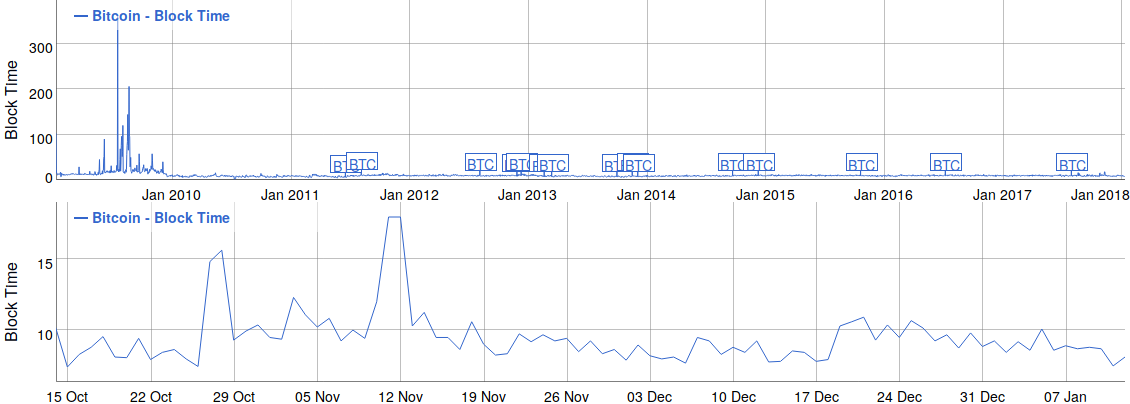
\includegraphics[width=\textwidth]{img/bitinfocharts-blocktime-btc}
%~ \caption[blocktime-btc]{\label{blocktime-btc}\mbox{Blockzeit f. Bitcoin}, \mbox{oben: Gesamt}, \mbox{unten: 6~Monate} %
%~ \mbox{Quelle: \cite{w:bitinfocharts}}
%~ } %\footnote{\url{https://bitinfocharts.com/comparison/bitcoin-confirmationtime.html}}
%~ \end{figure}

%~ Am Bsp. Bitcoin Abb.\,\ref{blocktime-btc} ist neben der Anfangsphase mit wenigen Teilnehmern eine stetige Schwankung über die Gesamte Laufzeit erkennenbar.

%~ Hierzur ist  zu sagen, dass eine größere Schwankung die geringere Wertung nach sich zieht,
%~ allerdingdings können die 

%~ \begin{figure}
%~ 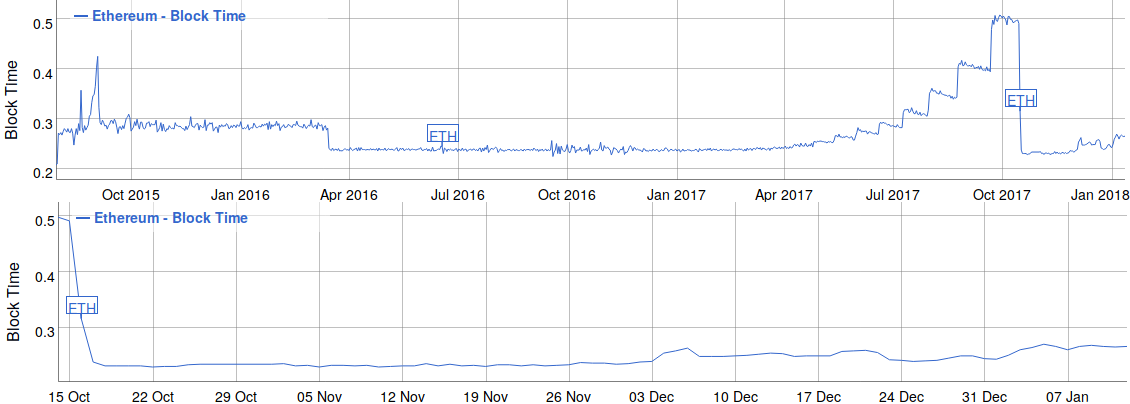
\includegraphics[width=\textwidth]{img/bitinfocharts-blocktime-eth}
%~ \caption[blocktime-eth]{\label{blocktime-eth}\mbox{Blockzeit f. Ethereum}, \mbox{oben: Gesamt}, \mbox{unten: 6~Monate} %
%~ \mbox{Quelle: \cite{w:bitinfocharts}}
%~ } %\footnote{\url{https://bitinfocharts.com/comparison/bitcoin-confirmationtime.html}}
%~ \end{figure}

%~ Bei Ethereum Abb.\,\ref{blocktime-eth} tritt eine ähnliche Auffälligkeit zur Anfangsphase auf.
%~ Zusätzlich sind sehr Deutlich Auswirkungen im März~2016\footnote{Homestead Release am 14.\,März~2016 \autocite{w:etherchain-hardforks}} und das Einsetzen der \enquote{Schwierigkeits-Bombe} (Engl. Difficulty-Bomb) bis zum abrupten Abfall\footnote{ab April~2017 (am Graph abgelesen) bis zum Byzantium Release am 16.\, Oktober~2017 \autocite{w:etherchain-hardforks}}. Beide Änderungen stehen je mit einer \gls{glos:Hard~Fork} in Verbindung.

%\begin{figure}
%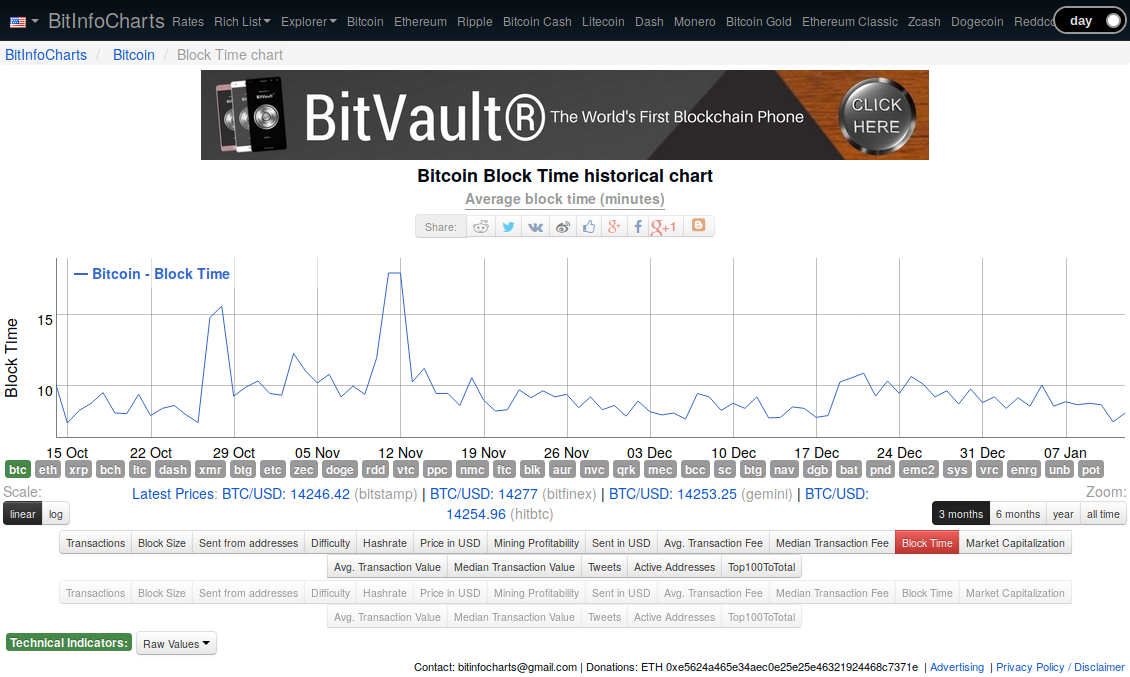
\includegraphics[width=\textwidth]{img/screenshot-bitinfocharts-2018-01-13-18-27-38}
%\end{figure}

%~ https://etherscan.io/chart/blocktime

%~ + Entwicklung von Kriterien
  %~ + Welche Eigenschaften bieten die Implementierungen
	%~ * Unterstützung
	%~ * Entwicklungsstand
	%~ * Kosten
	%~ * 
  %~ + Welchen Anwendungsfällen sind sie zu-/abträglich
	%~ * Viele Transaktionen
	%~ * Privatsphäre
	%~ * Integration Bestehender IT

%%
\section{Wirtschaftliche Gesichtspunkte}\label{krit:oeconomics}

Bevor naheliegende Kosten betrachtet werden, soll auch auf die Ertragsseite der Wirtschaftlichkeitsbetrachtung hingewiesen werden.
Die Bewertung ist sehr stark vom Einzelfall mit vielen Einflussfaktoren abhängig und wird daher in der Arbeit nicht als Kriterium aufgenommen.
Was Wertung von Angaben zu Kosten und Erträgen angeht, so sind höhere Kosten immer schlechter zu werten und höhere Erträge besser.

\subsection{Personalverfügbarkeit}\label{krit:personal}

Noch heute erscheint die Neuerung durch die \gls{BCT} so groß, dass der Bedarf an Personal nicht gedeckt ist.
%Aber ähnlich die Geometrie sind die Kenntnisse dahinter nur auf Zeit Spezialwissen.
Umso mehr Anwendungen den Alltag beeinflussen, umso mehr Informationen öffentlich zugänglich sind, desto leichter wird es sein diese Kompetenzen am Markt zu erhalten.
Bisweilen haben Firmen aber genau das Problem ihren Bedarf am Markt zu decken.

Die Betrachtung stellt auf die Verfügbarkeit von Personal und damit die Durchführbarkeit beabsichtigter Projekte ab und beinhaltet noch nicht die Kosten. 
%~ Daher spielt der Faktor Personal noch eine enorme Rolle bei initialen (horizontale Weiterbildung) und vor allem laufenden Kosten für Gehälter.
Die Wertung für geringere Personalverfügbarkeit ist kleiner als die höherer.

\subsection{Beschaffungskosten}\label{kosten}

%~ (gewonnen aus \nameref{first:kosten})
Für die Verwendung im konkreten Unternehmen notwendigen Einmalaufwendungen können eine wesentliche Zugangshürde zu Technologie darstellen.
Dies kann auch trotz \emph{offener Standards} und Open~Source Software der Fall sein wenn einzelne Akteure ihre Position oder ihren Wissensvorsprung monetarisieren.
Initiale Kosten können insbesondere Anschaffung von Hardware und ggf. Lizenzkosten\footnote{Bsp. Softwarelizenzen, Nutzungslizenz für Patente; auch Konzessionen wie die \emph{BitLicense} \autocite{w:bitlicense}} darstellen.
Auch andere Einmalaufwendungen -- \zB{} für den Zugang zu Verbänden -- zählen hierzu.

BigchainDB hat keine Preisliste, ist aber gesprächsbereit sofern Interesse an Beratung besteht.
Bei Hyperledger ist die intensive Mitarbeit für gewinnorientierte Unternehmen Gebührenpflichtig.
Gemeinnützige Organisationen können sich für eine kostenlose Mitgliedschaft bewerben.

\subsection{Laufende Kosten}

Abgesetzt von den Beschaffungskosten sind auch laufende Kosten zu betrachten.
Hier insbesondere Beiträge zu Verbänden und auf die \gls{BCI} beziehbare Personalkosten (s.a. \ref{krit:personal}) wie Gehälter und Weiterbildung.

%~ (gewonnen aus \nameref{first:regulierung})
Abgesehen von den Kosten ist auch die Beeinflussung des Umfeldes durch
Standardisierung und Regulierung (\label{regulierung}s. \ref{first:regulierung}) für Unternehmen eine Herausforderung.
Dabei können Kosten unregelmäßig auftreten und unvorhersehbar auftreten.

\subsection{Organisation}

Die Wirtschaftliche Organisation ist vergleichbar mit der \nameref{krit:community} (\ref{krit:community}).
Auch auf der Ebene der Betreiber soll eine Absicherung nicht vernachlässigt werden.
Ähnlich einem zentralen Entwickler kann eine zentrale Organisation ein Risiko für das Vertrauen darstellen.
Üblich sind inzwischen gemeinnützige Stiftungen, die die Weiterentwicklung einer Implementation und des Ökosystems darum sicherstellen sollen.
Diese ermöglichen auch eine Beteiligung weiterer -- natürlicher wie juristischer -- Personen.

Eine gemeinnützige Organisationsform ist ggü. einer gewinnorientierten hinsichtlich des in sie gesetzten Vertrauens besser zu werten.
Teilnahme-/Zugangsbeschränkung und Gleichheit können innerhalb einer solchen Organisation als zusätzliche Wertungsmöglichkeit herangezogen werden.


\chapter{Quantifizierung der Bewertung}
%~ + Quantifizierung der Bewertung
  %~ + Wertebereiche
  %~ + Klassifizierung
%~ + Darstellung
  %~ + 

%Methode: paarweiser Vergleich
Um die in Frage stehenden Blockchain-Implementierungen miteinander vergleichen zu können,
soll den eigenen Kriterien jeweils ein von der Software unabhängiges Gewicht als Präferenz für die Wichtigkeit zugeordnet werden.

Spezifisch für jedes Kriterien 
  
\chapter{Darstellung zur Präsentation}
%Methode: paarweiser Vergleich
%~ Um die in Frage stehenden Blockchain-Implementierungen miteinander vergleichen zu können,
%~ soll den eigenen Kriterien jeweils ein von der Software unabhängiges Gewicht als Präferenz für die Wichtigkeit zugeordnet werden.

%~ Spezifisch für jedes Kriterien 

Der Vergleich der gewonnen Kriterien soll nicht nur der Entscheidungsfindung dienen, sondern auch der Kommunikation der Entscheidung.
%~ Komplexität ist hier ein Gegenpol zur Nachvollziehbarkeit.
Nicht nur um sie nachvollziehbar zu machen, sondern auch weil im Zweifel mehrere Entscheider Einfluss nehmen möchten.
Daher steht die Frage der Darstellung hier im Vordergrund der Kommunikation.

Eine Wertung in Zahlen macht die Vergleichbarkeit einfacher.
Die Zuordnung von Attributen zur Abstufung nicht-binärer Bewertungen ist der Kommunikation zuträglich.
Da die einzelnen Kriterien in unterschiedliche -- weitgehend atomare -- Aspekte zerfallen können diese einzeln bewertet zur quantitativen Gesamtbewertung eines Kriteriums akkumuliert werden.
%~ \footnote{ \autocite{p:vergleich}}


\section{Optionen zur Darstellung}\label{depiction}

Entscheidungsprozesse müssen nicht nur innerhalb einer \gls{BC} nachvollziehbar sein.
Gerade in Unternehmen ist die Dokumentation und ggf. Wiederholbarkeit -- \zB{} im Rahmen des betrieblichen Benchmarking -- von gesteigertem Wert für den dauerhaften wirtschaftlichen Erfolg über den Einsatzzeitraum eines IT-Systems hinaus.

\subsection{Checklisten}

Eine sehr einfache und vielfältig gestaltbare Möglichkeit stellen Checklisten dar.
Sie kann zur Überprüfung von binären Kriterien kann sehr einfach im Sinne von erfüllt/nicht erfüllt \enquote{abgehakt} werden.

%~ die eigenschaft btf oder nicht und in klassen 2/3 oder 1/2
Wenn das Kriterium Konsens auf die für den Anwendungsfall notwendigen Aspekte reduziert wird kann ein Vergleich vorgenommen werden, welche \gls{BCI} das Kriterium insgesamt besser/schlechter/gleich erfüllt.\footnote{\cite{TN_libero_mab215408815}}

%~ \textbf{Beispielhaft eine Checkliste für das Kriterium \namref{krit:consensus} (\ref{krit:consensus})}
\begin{itemize} \setlength\itemsep{0em}\setlength\parskip{0em}\setlength\topsep{0em}\setlength\partopsep{0em}\setlength\parsep{0em}
\item Finalität
\item \gls{BFT}
\item Austauschbarkeit
\item Erlaubnisfreiheit
\item Dezentralität
\end{itemize}

Diese Darstellung eignet sich nicht für komplexere, multikriterielle Vergleiche.
Allein die Länge der Checkliste macht die Bewertung schnell unübersichtlich und eignen sich daher eher für die Unterstützung der Abarbeitung eines Vorgangs denn für die Entscheidungsfindung.

\subsection{Entscheidungsquadrat}

Eine Darstellung im Entscheidungsquadrat erschöpft sich bereits bei zwei Dimensionen, eine dritte erweitert bereits zum Würfel und führt zu einer schlechteren Ablesbarkeit.
Häufig werden die Dimensionen \enquote{dringlich} und \enquote{wichtig} verwendet; also eine Entscheidung zur Priorisierung unterstützt.
%~ Um die Entscheidungsstruktur in Unternehmen besser abzubilden, werden die Faktoren umgewidmet auf Preis und Relevanz.
Damit eignet sich das Entscheidungsquadrat in dieser Form \zB{} zur Unterstützung für geplante aber noch nicht verfügbare Eigenschaften einer \gls{BCI}.
%~ Dabei wird der Zeitfaktor 

\subsection{Ranking}\label{dep:ranking}

Die Wertungen werden in einer Dimension auf- oder absteigend geordnet. Eventuelle gleiche Wertungen können auftreten, sodass keine eindeutige Reihenfolge zustande kommt.
Die einfache Bewertung ohne Attributen oder Zahlen kann mit einer Rangfolge zum Ausdruck gebracht werden; d.h. eine Quantifizierung in Zahlen ist nicht unbedingt notwendig.
Im umgekehrten Fall, der Darstellung einer bereits mit Zahlen bewerteten oder auch in ihrem Rang definierten Attributen, ist lediglich noch eine verdeutlichende Wirkung zu erwarten.

Sofern eine quantitative Gesamtbewertung vorliegt, eignet sich das Ranking für die Darstellung der naheliegendsten \gls{BCI}.
Die Erstellung ist aber schwer nachvollziehbar und deshalb auch hinsichtlich der Wiederholbarkeit fehleranfällig.

\subsection{Paarweiser Vergleich}\label{dep:pugh}

Der Paarweise Vergleich (auch Pugh~Matrix) ermöglicht einen strukturierten Vergleich für eine beliebige Anzahl von Parametern.
Dabei werden die Kriterien horizontal und vertikal in eine Tabelle (Abb.\,\ref{abb:pugh-matrix}) eingetragen.
Die horizontale Addition der Wertungen kann als eine Rangwertung genutzt werden.\footnote{\cite{TN_libero_mab21000123709}}

\begin{figure}[!htp]
\centering
\begin{tabular}{|r||r|r|r|r|r|r||r|}
\hline
\(K_i\)	& 0 	& 1 	& 2 	& 3 	& 4 	& 5	& \(\sum{}\)\\
\hline \hline
0		& --	& 0		& 1		& 2		& 0		& 1	& 4			\\
\hline
1		& 2		& --	& 0		& 1		& 2		& 0	& 5			\\
\hline
2		& 1		& 2		& --	& 1		& 2		& 0	& 6			\\
\hline
3		& 0		& 1		& 1		& --	& 1		& 2	& 5			\\
\hline
4		& 2		& 0		& 0		& 1		& --	& 0	& 3			\\
\hline
5		& 1		& 2		& 2		& 0		& 2		& --& 7			\\
\hline \hline
\(\sum{}\) & \multicolumn{6}{r||}{} & {30} \\
\hline
\end{tabular}
\captionof{figure}[Beispiel Pugh Matrix]{\label{abb:pugh-matrix} Beispiel Paarweiser Vergleich der Kriterien}
\end{figure}

Die Zellen werden nun mit den Wertungen bis zu einem Maximum \(m \ge 2\) aus der Menge von Wertungsmöglichkeiten \(M\) für den direkten Vergleich von zwei sich kreuzenden Kriterien befüllt.
Dazu wird eine Zahl \(w \in [0;m] \)  höher für eine stärkere Wertung des Kriteriums in der Zeile vergeben, und geringer für eine stärkere Wertung des Kriteriums in der Spalte.
Die Diagonale in der das gleiche Kriterium mit sich selbst verglichen würde, entfällt und alle Vergleiche unterhalb der Diagonale sind invers zu den oberen Werten und können schlicht als \(w' = m - w\) am Maximalwert \(m\) gespiegelt werden.
Um eine neutrale Wertungen zum Ausdruck bringen zu können, muss die Menge \(M\) eine ungerade Anzahl an Möglichkeiten für \(w\) vorgeben.

Auch die Beteiligung mehrerer Entscheider ist die Kombination durch ein Produkt der einzelnen Bewertungen mehrstufig umsetzbar.
Eine Unterstützung durch \zB{} eine Tabellenkalkulation ist machbar, aber mit manuellen Aufwand für Anpassungen verbunden.
Jeder einzelne Bewertungsvorgang bleibt aufwändig -- und der Aufwand steigt exponentiell mit der Anzahl der Kriterien.
Damit ist das Bewertungsverfahren nicht gut geeignet in einem Meeting mit überschaubarem Zeitrahmen durchgeführt zu werden.

\subsection{Netzdiagramm}\label{dep:web}

Das Netzdiagramm (auch Radardiagramm, Kiviat-Diagramm, oder Sterndiagramm) besteht aus mindestens drei unabhängigen Parametern als Strahlen (für die quantitative Wertung der Kriterien) ausgehend von einem gemeinsamen Mittelpunkt in einer Darstellung (Abb.\,\ref{disp:web:pic}).

\begin{figure}[!htp]
%~ \scalegraphics{img/disp-web}
\centering
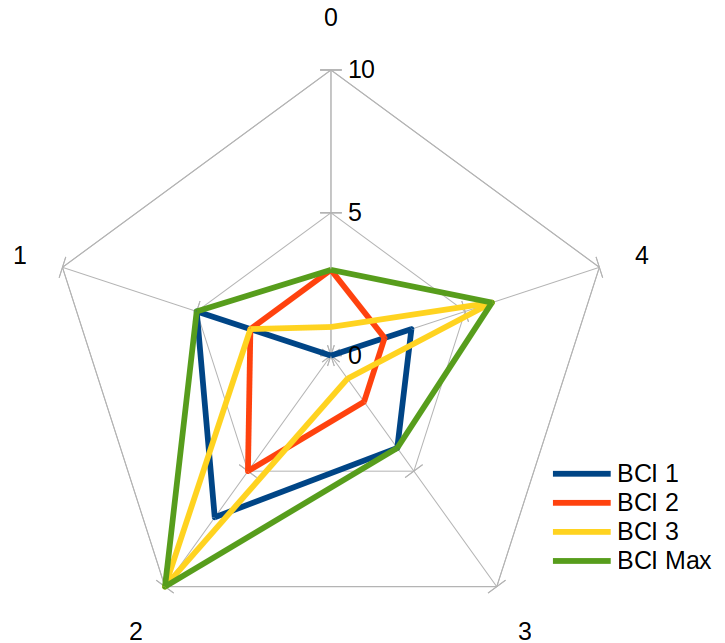
\includegraphics[width=.6\textwidth]{img/disp-web}
\captionof{figure}[Beispiel Netzdiagramm]{\label{disp:web:pic} Beispiel Netzdiagramm}
\end{figure}

Abhängig vom Radius der Abbildung lässt sich so leicht eine zweistellige Anzahl von Parametern einbringen;
optimal ist die Darstellung jedoch eher für 5-7 Kriterien.
Eine mehrdimensionale Darstellung wie das Netzdiagramm eignet sich um die Parameter einer \gls{BCI} in einer Abbildung zusammenzufassen.
%~ Sowohl Gegensätze als auch Skalierungen können so verdeutlicht werden.
Die Fläche des Vieleckes, dass sich aus den am je abgezeichneten Strahlen verbundenen Schnittpunkten ergibt, steht sowohl mit ihrem Betrag als auch dem optischen Eindruck für die Bewertung der damit illustrierten \gls{BCI}.
Für die Darstellung und auch Berechnung ist eine gleichwinklige Verteilung der Strahlen hilfreich.

Die exakte Erstellung ist manuell nicht trivial; dank der simplen geometrischen Regeln aber leicht mit \ua{} einer Tabellenkalkulation zu realisieren.
Soweit die Wertreihe für unterschiedliche \gls{BCI} voneinander abweichen, lassen sich auch zwei oder mehr Wertreihen in einer Abbildung zusammen fassen.

Unabhängig von der grafischen Erstellung kann die Berechnung vorgenommen werden.
Die Fläche \(F\) zerfällt in Dreiecke um den Mittelpunkt \(C\) bei denen jeweils die Seiten \(a, b\) und der Winkeln \(\gamma\) bekannt sind.

\[
F_{\text{Dreieck}} = \frac{ab\sin{\gamma}}{2}
\text{\hspace{2em}}\Rightarrow{}\text{\hspace{2em}}
F_{n\text{-Eck}} = \sum_{i=0}^{n} \frac{a_{i} b_{(i+1)\mod n} \sin{\gamma}}{2}
\]

Da die Winkel im gleichwinkligen \(n\)-Eck mit %\(\gamma\) für
\( \frac{\tau}{n}\ = \frac{2\pi}{n}\) bzw. \(\frac{360^\circ{}}{n}\) konstant sind,
kann die Berechnung der Entscheidungsgrundlage \(E\) für jeden Sektor vereinfacht werden.
Die Summe ist unter Beachtung der Grenzen dann ebenfalls leichter zu ermitteln.

\[
E_{\text{Sektor}} = ab 
\text{\hspace{2em}}\Rightarrow{}\text{\hspace{2em}}
E_{gesamt} = \sum_{i=0}^{n} a_{i} b_{(i+1)\mod n}\text{\hspace{3em}}\Big|{\gamma \text{ konstant}}
\]

Da der exakte Wert der Fläche nicht relevant ist, sondern das Verhältnis zu einem theoretischen Pareto Optimum,
kann dieses durch die Maximalwerte alle betrachteten \gls{BCI} gebildet werden.
Die einzelnen -- im Grunde wegen der Nichtaustauschbarkeit zwischen den \gls{BCI} -- nicht miteinander vergleichbaren
Kandidaten können jedoch über das Verhältnis mit dem Pareto Optimum miteinander verglichen werden.


%~ \section{Anwendung auf die Kriterien}

\section{Quantifizierung}

Die Quantifizierung -- also Bewertung in Zahlen -- der bisher durch Beschreibung (in Worten) durchgeführten subjektiven Bewertung soll das Verständnis für die Wertigkeit klarer zum Ausdruck bringen und ggf. eine Berechnung ermöglichen.
In jede Fall kann dadurch eine objektivere Sicht bzw. die Begründung für Anpassungen eingebracht werden.

%~ Als Beispiel dient hier die Bewertung 

\subsection{Gruppierung}

In der Wertung haben manche Kriterien eine höhere Priorität als andere.
Die Gruppierung ermöglicht die Konzentration auf diese Prioritäten und thematische Zusammenhänge.
%~ An dieser Stelle können die unterschiedlichen Wertebereiche auch gezielt mit einem weiteren Faktor ausgeglichen werden.

Die Einteilung kann genutzt werden um Schwerpunkte für den eigenen Anwendungsfall zu setzen,
%~ \begin{enumerate}
einzelne Kriterien hinsichtlich der Wertung an- oder abzuwählen und sich auf die für eigene Zwecke notwendigen Gruppen zu konzentrieren.
Die Einteilung sollte für den Bewertungsprozess \zB{} dadurch hilfreich sein, dass unterschiedliche Spezialisten eine Teilentscheidung beitragen können.
Die Kriterien wurden beispielhaft in den drei Gruppen \nameref{krit:it} (\ref{krit:it}), \nameref{krit:blockchainproperties} (\ref{krit:blockchainproperties}) und \nameref{krit:oeconomics} (\ref{krit:oeconomics}), zusammengefasst.
%~ \end{enumerate}

\subsection{Klassifizierung}\label{classification}

Die in Worte gefasste Einteilung kann entlang des Wertungsgefälles mit Zahlen belegt werden.
Die einfachste Art von Klassen definieren sich durch Grenzen.
Jedoch ist der Übergang nicht immer eindeutig abgestuft.
Um das Problem handhabbar zu machen, wird vorgeschlagen die Unterteilung in binär beantwortbare Aspekte vorzunehmen.
Diese sollten mindestens so weit erweitert werden, wie es für die eigenen Zwecke notwendig ist.
Optimal wäre eine Erweiterung um Bedingungen bis die zu vergleichenden Kandidaten unterscheidbar werden.
Eine darüber hinausgehende Unterscheidung bedeutet lediglich mehr Arbeit in der Auswertung ohne einen direkten Nutzen; kann aber für eine künftige Iteration als vorbereitende Maßnahme wichtig sein.

Als Beispiel hierfür sei die Klassifizierung von Software-Lizenzen (s.a. \ref{krit:opensource}) angeführt.
Die Aspekte könnten sein:

%~ \begin{itemize}
%~ \item Verwendungserlaubnis ohne Einschränkungen
%~ \item Lesen der Quellen ohne Vorbedingunen
%~ \item Verteilen von Kopien
%~ \item 
%~ \end{itemize}

\begin{enumerate} \setlength\itemsep{0em}\setlength\parskip{0em}\setlength\topsep{0em}\setlength\partopsep{0em}\setlength\parsep{0em}
\item Open~Source gem. OSI (vgl. \ref{krit:opensource})
\item Behandlung von Software-Patenten
\item Gleiche Garantien auch ohne Auslieferung einer Software (\zB{} Webservice)
\item Veränderung ist trotz \gls{DRM} garantiert
\end{enumerate}

Damit lassen sich die Lizenzen der behandelten Kandidaten in Wertungen 0/1 (nein/ja) unterscheiden.

\begin{figure}[!htp]
\centering
\begin{tabular}{l|lll}
Aspekt	& LGPL\,3.0 	& Apache~License\,2.0 & AGPL\,3.0 \\
\hline
\hline
1 		& 1	& 1	& 1	\\
\hline
2 		& 1	& 1	& 1	\\
\hline
3 		& 0	& 0	& 1	\\
\hline
4		& 1 & 0 & 0 \\
\hline
\hline
\(\sum\)& 3 & 2 & 3 \\
\end{tabular}
\captionof{figure}[Beispiel Wertung Softwarelizenzen]{\label{abb:wertung:oss} Beispiel einfache Wertung von Softwarelizenzen}
\end{figure}

\subsection{Gewichtung}

Das gleiche Ergebnis (\nameref{classification}, Abb.\,\ref{abb:wertung:oss}) für die LGPL\,3.0 und die AGPL\,3.0 in der Summe verdeutlicht,
dass vollständiger Unterscheidbarkeit das Ergebnis nicht eindeutig sein muss.

Um das Problem zu verringern, ist eine Gewichtung hilfreich.

\subsubsection*{Begründung am Beispiel}
Wir gewichten hier die Aspekte 2-4 höher weil sie für die unternehmerische Nutzung von gesteigerter Bedeutung sind.
Aspekt 1 wird nicht höher gewichtet, da es sich um das im technologischen Umfeld übliche Mindestmaß handelt, das auch eingehalten wird.
Wegen des primären Einsatzes von Webtechnologien und der daraus resultierenden Verwendung von Services in Netzwerken bei gleichzeitiger Kommplung mit der \gls{BCT}, die selbst auf Netzwerken basiert, wird Aspekt 3 nochmals stärker gewichtet.

\begin{figure}[!htp]
\centering
\begin{tabular}{l|llll}
Aspekt	& Gewichtung & LGPL\,3.0 	& Apache~License\,2.0 & AGPL\,3.0 \\
\hline
\hline
1 		& 1	& 1	& 1	& 1	\\
\hline
2 		& 2	& 2	& 2	& 2	\\
\hline
3 		& 3	& 0	& 0	& 3	\\
\hline
4		& 2	& 2 & 0 & 0 \\
\hline
\hline
\(\sum\)& --& 5 & 3 & 6 \\
\end{tabular}
\captionof{figure}[Beispiel Gewichtete Wertung]{\label{abb:wertung:oss2} Beispiel Gewichtete Wertung von Softwarelizenzen}
\end{figure}

Durch die Stärkere Gewichtung der möglicherweise geschäftskritischeren Fragen kann damit ein eindeutiges Ergebnis für das Kriterium ermittelt werden.
Wichtig für die Nachvollziehbarkeit ist die Dokumentation des Grundes für eine Gewichtung.

\subsection{Entscheidungsunterstützung}

Das verkürzte Beispiel zu den Software (Abb.\,\ref{abb:wertung:oss2}) lässt sich nun einfach per \nameref{dep:ranking} (\ref{dep:ranking}) entscheiden.
Der Nutzen der Abbildung nur eines Kriteriums ist jedoch sehr begrenzt.

Da Entscheidungen sehr leicht subjektiv werden sind die Maßnahmen zur Gruppierung, \nameref{classification} und Gewichtung entscheidend um
eine objektive und nachvollziehnbare Grundlage zu erreichen.

Der Paarweise Vergleich (\ref{dep:pugh}) kann mehrstufig eingesetzt zu einer guten Entscheidungsgrundlage führen.
Der mit Anzahl der Kriterien wachsende Aufwand und die geringe Eignung für die direkte bildliche Darstellung begrenzen den praktischen Nutzen.

Dagegen kann durch das \nameref{dep:web} (\ref{dep:web}) eine gute grafische Darstellbarkeit -- für sogar mehrere Kandidaten -- in einem Bild aufweisen.
Zusätzlich ist die Berechenbarkeit eines Entscheidungskriteriums und die Vergleichbarkeit mit einem Pareto-Optimum ein entscheidender Vorteil sowohl was die Einschränkungen für Präsentationen bei Entscheidern betrifft als auch die Argumentation bezüglich des theoretisch erreichbaren.



\chapter{Fazit und Ausblick}
\cleardoublepage 

\pagenumbering{Roman} %for non-content

%~ * Anhang
  %~ + Literaturverzeichnis
  %~ + Ehrenwörtliche Erklärung

% TOC ergänzen, bib bauen
\printbibliography[title={Quellennachweise%\\\hspace{1mm}\,\\\normalfont{}\normalsize{}\quellenHinweistext{}%
}]
\addcontentsline{toc}{chapter}{Quellennachweise}
\cleardoublepage 

\appendix
%~ \chapter*{Anlagen}
%~ \addcontentsline{toc}{chapter}{Anlagen}
%~ \addstarredchapter{Anlagen}
%~ \minitoc
%~ \clearpage

%~ \addsec{Vorgehen mit VirtualBox}\label{apx:vb}
%~ \input{vb}
%~ \clearpage

% externe pdf einbinden
%~ \addcontentsline{toc}{section}{Organisationsplan der TU Dresden}%\addsec{Organisationsplan der TU Dresden}
%~ \label{apx:tud}
%~ \includepdf[landscape=true,pages=-]{dat/Organisationsplan_TUD.pdf}
%~ \clearpage


%~ + Ehrenwörtliche Erklärung
\hspace{1mm}\,\vspace{3em}
\addsec{Selbstständigkeitserklärung}\label{apx:ee}
%\section*{Selbstständigkeitserklärung}

Ich versichere, dass die vorgelegte Arbeit selbstständig verfasst und keine anderen als die angegebenen Quellen und Hilfsmittel genutzt wurden.


\WritePlace{}, \DocDate{}\\
\,\hspace{1cm}\Author{} \\

\clearpage


\end{document}
